\section{Ergebnisse}
\subsection{Beteiligung}

Bei der Erhebung der Winterverluste 2019/20 haben wir von 1.539 Imkereien Datensätze zu 30.724 eingewinterten Bienenvölkern erhalten. Prozentual betrachtet erreicht die Beteiligung österreichischer Imkereibetriebe dabei einen Wert von 5,1\%. Diese gaben Rückmeldung über 7,9\% aller in Österreich gehaltenen Bienenvölker. In der nachstehenden \cref{tab:u:beteiligungsrate} werden auch die Rückmeldungen der vorangegangenen Winter dargestellt. Die Grundlage für die Berechnung der Rückmeldungen (in \%) bilden die Daten der „Biene Österreich`` (\cref{tab:u:beteiligungsrate}).

\begin{table}[H]
    \caption{Beteiligungsrate der österreichischen Imkereien an unserer Umfrage zu den Winterverlusten seit Winter 2013/14.}
    \label{tab:u:beteiligungsrate}
    \begin{tabular}{c|*{2}{r}r|*{3}{r}}
        %%\hline
        \multicolumn{1}{c}{}&
        \multicolumn{3}{c}{Imkereien} & 
        \multicolumn{3}{c}{Bienenvölker} \\
        \cline{2-7}
        \multicolumn{1}{c}{Jahr} & 
        \makecell{Gesamt$^1$ [\#]} &
        \makecell{Teilnehmer [\textit{n}]} &
        \makecell{Anteil [\%]} &
        \makecell{Gesamt$^1$ [\#]} &
        \makecell{Teilnehmer$^2$ [\textit{n}]} &
        \makecell{Anteil [\%]} \\ 
        \hline
        2013/14 & 25.492 & 1.023 & 4,0 & 382.638 & 18.794 &  4,9 \\
        2014/15 & 25.277 & 1.259 & 5,0 & 376.121 & 22.882 &  6,1 \\
        2015/16 & 26.063 & 1.289 & 4,9 & 347.128 & 23.418 &  6,7 \\
        2016/17 & 26.609 & 1.656 & 6,2 & 354.080 & 43.852 & 12,4 \\
        2017/18 & 27.580 & 1.391 & 5,0 & 353.267 & 28.373 &  8,0 \\
        2018/19 & 28.432 & 1.534 & 5,4 & 373.412 & 33.651 &  9,0 \\
        2019/20 & 30.237 & 1.539 & 5,1 & 390.607 & 30.724 &  7,9 \\
        \hline
    \end{tabular}
    \scriptsize
    $^1$Die angeführten Gesamtzahlen beziehen sich auf Imkereien und Bienenvölker in Österreich und beruhen auf Angaben der \enquote{Biene Österreich}. Diese Zahlen bilden die Grundlage für die Berechnung der Rückmeldungen. 
    \\
    $^2$Gesamtsumme der eingewinterten Bienenvölker der teilnehmenden Imkererein.
\end{table}



\subsection{Repräsentativität}
\subsubsection{Anonyme Teilnahme versus nicht anonyme Teilnahme}

Von den 2019/20 insgesamt 1.539 Imkereien haben 503 (32,7\%) anonym teilgenommen während 1.036 (67,3\%) eine Kontaktmöglichkeit (Kontaktadresse, E-Mail oder Telefonnummer) hinterlassen haben. Beim Vergleich der Verlustrate zwischen anonymen \confi{13,1}{95}{11,8}{14,7} und nicht-anonymen Teilnehmern \confi{12,4}{95}{11,6}{13,3} konnte in diesem Jahr kein signifikanter Unterschied festgestellt werden (\cref{fig:u:anonymity}).

\myfig{project-U-wintersterblichkeit/figures/plot_anonymity} % Pfad
  {width=0.6\textwidth} % Größe Relativ zu Text Breite
  {Höhe der Winterverluste 2019/20 anonymer TeilnehmerInnen und nicht-anonymer Teilnehmer\-Innen in Prozent (±95\%KI).} % Text unterhalb der Grafik
  {Optionaler Kurz Titel} % Optional Kurz Überschrift
  {fig:u:anonymity} % Label zum Verweisen im Text
  

\subsubsection{Online-Antworten versus Papierfragebogen-Antworten}

Die Teilnahme war online, mittels Papierfragebogen oder mittels Kurzfragebogen in der Zeitschrift „Biene Aktuell`` möglich. \cref{tab:u:teilnameart} zeigt, wie viele ImkerInnen sich von 2013/14 bis 2019/20 online, auf Papier oder über die Zeitschrift an unserer Untersuchung beteiligt haben. Die meisten Antworten erreichten uns online (\cref{tab:u:teilnameart}). Heuer war eine signifikante höhere Verlustrate bei Zeitschriften-TeilnehmerInnen \confi{18,7}{95}{14,7}{23,3} im Gegensatz zu Online-TeilnehmerInnen \confi{12,3}{95}{11,5}{13,0} zu erkennen. Personen die Papierfragebögen eingeschickt haben, zeigten keinen signifikanten Unterschied zu den zwei anderen Gruppen \confi{13,9}{95}{11,1}{17,3} (\cref{fig:u:onlinevspaper}). 

\myfig{project-U-wintersterblichkeit/figures/plot_onlinevspaper} % Pfad
  {width=0.6\textwidth} % Größe Relativ zu Text Breite
  {Höhe der Winterverluste 2019/20 der unterschiedlichen Teilnahmearten (online, Papier, Zeitung) in Prozent (±95\%KI).} % Text unterhalb der Grafik
  {Optionaler Kurz Titel} % Optional Kurz Überschrift
  {fig:u:onlinevspaper} % Label zum Verweisen im Text

\begin{table}[H]
    \centering
    \caption{Art der Teilnahme an der Erhebung der Winterverluste von 2013/14 bis 2019/20 (Anzahl TeilnehmerInnen (\%)).}
    \label{tab:u:teilnameart}
    \begin{tabular}{c|*{2}{rr|}rr}
        \toprule
            \multicolumn{1}{c}{}& 
            \multicolumn{2}{c}{Internet} & 
            \multicolumn{2}{c}{Papier} & 
            \multicolumn{2}{c}{Zeitschrift} \\
        \cmidrule{2-7}
            \multicolumn{1}{c}{Jahr} & 
            \multicolumn{1}{c}{\textit{n}} & 
            \multicolumn{1}{c}{\%} & 
            \multicolumn{1}{c}{\textit{n}} & 
            \multicolumn{1}{c}{\%} & 
            \multicolumn{1}{c}{\textit{n}} & 
            \multicolumn{1}{c}{\%} \\
        \midrule
        2013/14 &   679 & 66,4 & 318 & 31,1 & 26 & 2,5 \\
        2014/15 &   947 & 75,2 & 249 & 19,8 & 63 & 5,0 \\
        2015/16 &   944 & 73,2 & 290 & 22,5 & 55 & 4,3 \\
        2016/17 & 1.268 & 76,6 & 332 & 20,0 & 56 & 3,4 \\
        2017/18 & 1.101 & 79,2 & 238 & 17,1 & 52 & 3,7 \\
        2018/19 & 1.378 & 89,8 &  93 &  6,1 & 63 & 4,1 \\
        2019/20 & 1.362 & 88,5 &  91 &  5,9 & 86 & 5,6 \\
        \bottomrule
    \end{tabular}
\end{table}

\subsubsection{Betriebsgröße}

Die Verteilung der Größen der teilnehmenden Betriebe ist in \cref{fig:u:betrieb}-A grafisch dargestellt. Für das Jahr 2019/20 liegt die durchschnittliche Anzahl der eingewinterten Bienenvölker aller teilnehmenden Imkereien bei 20 Völker pro Imkerei. Das ist etwas mehr als der österreichweit erwartete Mittelwert (\enquote{Biene Österreich}, ca. 13 Völker/Imkerei). Dies kommt durch die Teilnahme von großen Imkereien mit jeweils über 150 eingewinterten Völkern und der daraus resultierenden ungleichen Verteilung der Bienenvölker in unserer Umfrage zustande (\cref{fig:u:betrieb}-B). Der Median der eingewinterten Völker liegt jedoch bei 10, was in etwa der österreichischen Imkerei-Demographie entspricht. 

\myfig{project-U-wintersterblichkeit/figures/plot_overview_betrieb} % Pfad
  {width=1\textwidth} % Größe Relativ zu Text Breite
  {Betriebsgröße der teilnehmenden Imkereien 2019/20. (A) Anzahl der Imkereien in den jeweiligen Betriebsgrößen. (B) Summe der eingewinterten Bienenvölker in den jeweiligen Betriebsgröße.} % Text unterhalb der Grafik
  {Optionaler Kurz Titel} % Optional Kurz Überschrift
  {fig:u:betrieb} % Label zum Verweisen im Text

\subsubsection{Geografische Herkunft}

\cref{fig:u:overviewmap} zeigt die ungefähre geografische Position des Haupt-Überwinterungsbienenstandes der TeilnehmerInnen, exklusive ImkerInnen deren Bienenstände über mehreren Bezirke verteilt sind. Die Karte zeigt eine landesweite Verbreitung über ganz Österreich, wobei einige Gebiete dominanter waren als andere. Dies könnte auf geografisch unzugängliche Gebiete wie Gebirgszüge zurückgeführt werden und Gebiete mit geringerer Dichte an Imkereibetrieben.

\myfig{project-U-wintersterblichkeit/figures/plot_overview_map} % Pfad
  {width=0.8\textwidth} % Größe Relativ zu Text Breite
  {Geografische Position des Haupt-Überwinterungsbienenstandes der an der Untersuchung der Winterverluste teilnehmenden Imkereien 2019/20. Aggregation der Standorte zu Punkten über eine modifizierte Kluster-Methode, siehe Sektion Material und Methoden.} % Text unterhalb der Grafik
  {Optionaler Kurz Titel} % Optional Kurz Überschrift
  {fig:u:overviewmap} % Label zum Verweisen im Text

\subsubsection{Bienenstandort}

Des Weiteren wurden die TeilnehmerInnen in unserer Erhebung gefragt ob sich all ihre Bienenvölker innerhalb eines \SI{15}{\kilo\meter} Radius zum angegebenen Winterstandort befinden. Diese Information ist wichtig für weitere standortbezogene Auswertungen in denen mögliche Zusammenhänge zwischen den Winterverlusten und dem Wetter, der Landnutzung sowie der Seehöhe näher betrachtet werden können.
\newline
In diesem Untersuchungsjahr gaben 88,3\% der TeilnehmerInnen an dass sich all ihre Bienenvölker innerhalb \SI{15}{\kilo\meter} des angegebenen Winterstandortes befanden. 11,0\% gaben an diesen Radius zu überschreiten. Nur 0,3\% der eingelangten Antworten entfielen auf die Kategorie „Unsicher`` und 0,4\% enthielten keine derartige Information.

\subsection{Verlustrate in Österreich, den Bundesländern und den Bezirken}
\subsubsection{Österreich}

Die teilnehmenden 1.539 Imkereien haben im Untersuchungsjahr 2019/20 insgesamt 30.724 Völker eingewintert. Seit Beginn der Erhebung schwanken die Winterverlustraten jährlich. Die Verlustrate aus dem Winter 2015/16 stellt mit \confi{8,1}{95}{7,4}{8,8} die niedrigste, jene aus dem Winter 2014/15 mit \confi{28,4}{95}{27,0}{29,9} die höchste seit Beginn der Erhebungen von Winterverlusten im Jahr 2007/08 dar (\cref{tab:u:states-year}). Die Winterverluste von Bienenvölkern über den Winter 2019/20 betrugen \confi{12,6}{95}{11,9}{13,3}. In \cref{fig:u:years:losses} werden, neben den diesjährigen gemessenen Verlustraten, auch die in den Jahren davor erhobenen Werte zum Vergleich dargestellt. Der langjährige laufende Mittelwert liegt bei 16,1\%, inkl. Winterverluste 2019/20.

\begin{figure}[H]
  \centering
  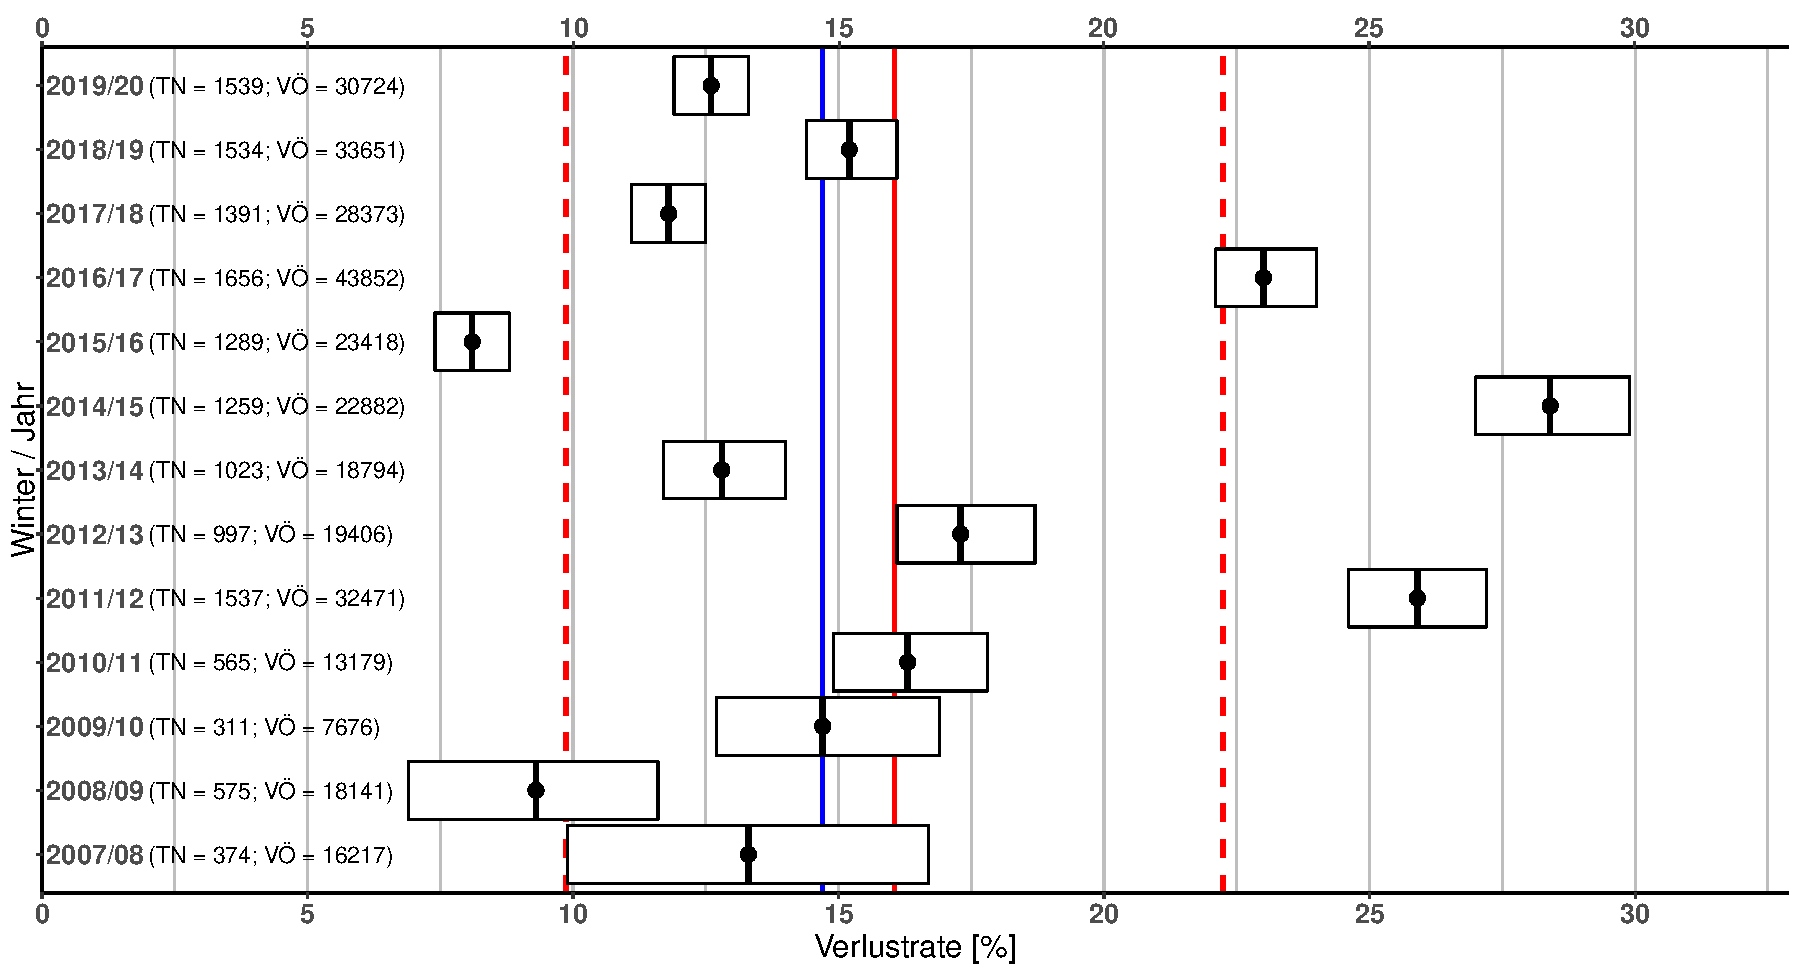
\includegraphics[keepaspectratio,width=1\textwidth]{project-U-wintersterblichkeit/figures/plot_years_losses}
  \caption{Höhe der Winterverluste in Österreich von 2007/08 bis 2019/20 in Prozent ($\pm$95\%KI). Rote Linie kennzeichnet den laufenden Mittelwert inkl. aktueller Umfrage; Rot strichlierte Linien ist die Standardabweichung vom Mittelwert. Blaue Linie kennzeichnet den Median Wert. TN = TeilnehmerInnen, VÖ = Gesamtsumme der eingewinterten Völker}
  \label{fig:u:years:losses}
\end{figure}

\subsubsubsection{Populationsdynamik in Österreich}

Die Berechnungen zur Populationsdynamik basieren auf den Angaben jener Imkereien, die auch die Anzahl ihrer Völker im Frühjahr des Einwinterungsjahres bekannt gegeben haben (Subpopulation). Mit Hilfe dieser Information konnte die Netto-Änderung der Population bis zum Herbst desselben Jahres (Einwinterungsvölker) berechnet werden. Die Zahl an Bienenvölkern im Frühjahr des Auswinterungsjahres konnte aus der Differenz zwischen eingewinterten und der im Winter verlorenen Völker berechnet werden. Dies berücksichtigt aber nicht etwaige im Winter zugekaufte oder verkaufte Völker, sowie die Netto-Änderung über den Sommer. Die Informationen zur Anzahl der Völker im Frühjahr, eingewinterten Völkern und zum Völkerverlust über den Winter des jeweiligen Jahres ermöglichen eine grafische Darstellung der Populationsdynamik österreichischer Bienenvölker vom Frühjahr 2013 bis zum Frühjahr 2020 (\cref{fig:u:population}).
\newline
Ausgehend von der Völkeranzahl im Frühjahr des Einwinterungsjahres stieg die Zahl an Bienenvölkern durch Vermehrung und Zukäufe jeweils bis zum Herbst an (\cref{tab:u:population}, „Vermehrung über den Sommer [\%]``). Die prozentuelle Änderung der Anzahl der Bienenvölker vom Frühjahr des Auswinterungsjahres zum Frühjahr des Einwinterungsjahres ist in \cref{tab:u:population} („Vergleich Frühjahr-Frühjahr [\%]``) zu finden. Allgemein zeigt sich, dass die Vermehrung im Sommer manchmal eine konstante, manchmal sogar eine wachsende Bienenpopulation ermöglicht (\cref{fig:u:population}). Welche Netto-Zuwachsrate erforderlich wäre, um nach dem Winter wieder auf den Stand der Bienenpopulation im Herbst des Einwinterungsjahres zu kommen, ist unter „Ausgleich Verluste [\%]`` ersichtlich. 
\newline
Die tatsächliche Netto-Vermehrung über den Sommer liegt für das Untersuchungsjahr 2019/20 um 5,8\% über der Schätzung des letzten Jahres, in der berechnet worden war, welche Netto-Zuwachsrate erforderlich gewesen wäre, um eine konstante Population zu ermöglichen.

\begin{table}[H]
    \caption{Populationsdynamik der Subpopulation (Imkereien mit vollständigen Angaben) untersuchter österreichischer Bienenvölker vom Frühjahr 2013 bis zum Frühjahr 2020.}
    \label{tab:u:population}
    \scriptsize
    \begin{tabular}{|c|*{8}{r|}}
        \hline
        & & & 
        \multicolumn{3}{c|}{Anzahl Bienenvölker} & & 
        \multirow{2}{*}{\shortstack{Vergleich \\ Frühjahr-\\Frühjahr[\%]}} & 
        \\
        \cline{4-6}
        Jahr & 
        \makecell{Imkereien \\ [\textit{n}]} & 
        \makecell{Verlust- \\ rate [\%]$^1$} & 
        \makecell{Frühjahr [\#]$^2$} & 
        \makecell{Eingewintert \\ Herbst [\#]} & 
        \makecell{Ausgewintert \\ Frühjahr [\#]} & 
        \makecell{Vermehrung \\ Sommer [\%]} & 
        & 
        \makecell{Ausgleich \\ Verluste [\%]$^3$} 
        \\
        \hline
        2013/14 &   973 & 12,9 & 14.319 & 17.816 & 15.518 & 24,4 &   8,4 & 14,8 \\
        2014/15 & 1.188 & 28,6 & 17.355 & 21.616 & 15.437 & 24,6 & -11,1 & 40,0 \\
        2015/16 & 1.195 &  7,9 & 15.102 & 21.800 & 20.070 & 44,4 &  32,9 &  8,6 \\
        2016/17 & 1.537 & 22,5 & 27.695 & 40.141 & 31.108 & 44,9 &  12,3 & 29,0 \\
        2017/18 & 1.285 & 11,6 & 18.983 & 25.670 & 22.695 & 35,2 &  19,6 & 13,1 \\
        2018/19 & 1.465 & 15,3 & 24.747 & 31.036 & 26.277 & 25,4 &   6,2 & 18,1 \\
        2019/20 & 1.478 & 12,5 & 23.802 & 29.484 & 25.802 & 23.9 &   8,4 & 14,3 \\
        \hline
    \end{tabular}
    \scriptsize
    $^1$ Verlustrate der teilnehmende Imkereien mit vollständigen Angaben zur Anzahl der Völker im Frühjahr des Einwinterungsjahres.
    \newline
    $^2$ Völker im Frühjahr des Einwinterungsjahres.
    \newline
    $^3$ Erforderliche Netto-Zuwachsrate, um nach dem Winter wieder auf den Stand der Bienenpopulation im Herbst des Einwinterungsjahres zu kommen.
\end{table}



\myfig{project-U-wintersterblichkeit/figures/plot_population} % Pfad
  {width=0.8\textwidth} % Größe Relativ zu Text Breite
  {Veranschaulichte Populationsdynamik von Bienenvölkern der Teilnehmer in Österreich vom Frühjahr 2013 bis zum Frühjahr 2020 basierend auf Winterverlusten und Vermehrung über den Sommer aus \cref{tab:u:population} Diese theoretische Entwicklung der Völkeranzahl basiert auf einer Ausgangszahl von 100 Völkern. Rote Punkte sind die Anzahl an Bienenvölkern im Frühjahr des angegeben Jahres und Blaue Punkte sind die Anzahl der Bienenvölker beim einwintern.} % Text unterhalb der Grafik
  {Optionaler Kurz Titel} % Optional Kurz Überschrift
  {fig:u:population} % Label zum Verweisen im Text

\subsubsection{Bundesländer}

Zwischen den Bundesländern sind die Völkerverluste nicht gleichmäßig verteilt. Hier zeigen sich besonders für Wien signifikant höhere Verluste von \confi{12,6}{95}{11,9}{13,3} im Vergleich zu den anderen Bundesländern (ausgenommen Burgenland) und im Vergleich zum österreichischen Gesamtverlust (\cref{fig:u:states}). Die \cref{tab:u:states} zeigt die Anzahl der teilnehmenden Betriebe, die Anzahl der eingewinterten Völker, die Anzahl der verlorenen Völker, Winterverluste aufgrund von Königinnen-Problemen und die Verlustrate in Summe und Prozent (inklusive 95\% Konfidenzintervall) für ganz Österreich und die einzelnen Bundesländer. Einen Überblick über die Winterverluste in ganz Österreich sowie in den Bundesländern für einen Untersuchungszeitraum von 6 Jahren, bietet die \cref{tab:u:states-year}. \cref{fig:u:states} zeigt eine grafisch Darstellung der mittleren Verlustraten anhand einer Österreich Karte.

\myfig{project-U-wintersterblichkeit/figures/plot_overview_states} % Pfad
  {width=0.8\textwidth} % Größe Relativ zu Text Breite
  {Höhe der Winterverluste 2019/20 für Österreich und die Bundesländer in Prozent ($\pm$95\%KI).} % Text unterhalb der Grafik
  {} % Optional Kurz Überschrift
  {fig:u:states} % Label zum Verweisen im Text

\begin{table}[H]
    \caption{Teilnehmende Imkereibetriebe, eingewinterte Völker und Verlustraten von Bienenvölkern im Winter 2019/20 für Österreich und pro
    Bundesland. Völkerverluste durch „Elementarschaden (Flut, Vandalismus, etc.)`` (\sample{181}) sind nicht inkludiert.}
    \centering
    \scriptsize
    \label{tab:u:states}
    \begin{tabular}{l*{7}{r}}
        \toprule
        \makecell{Bundesland} &
        \makecell{Teilnehmende \\ Imkereien [n]} &
        \makecell{Völker \\ eingewintert[n]} &
        \makecell{Tote \\ Völker [n]} &
        \makecell{Verluste \\ (Königinnen-\\Probleme) [n]} &
        \makecell{Summe \\ Verlust [n]} &
        \makecell{Verlust \\ {[\%]}} &
        \makecell{CI {[\%]}} \\
        \midrule
        Österreich       & 1.539 & 30.724 & 2.539 & 1.334 & 3.873 & 12,6 & 11,9 - 13,3 \\
        Burgenland       &    33 &    521 &    31 &    23 &    54 & 10,4 &  6,3 - 16,6 \\
        Kärnten          &   151 &  3.743 &   338 &   140 &   478 & 12,8 & 10,8 - 15,0 \\
        Niederösterreich &   389 &  8.085 &   734 &   408 & 1.142 & 14,1 & 12,7 - 15,7 \\
        Oberösterreich   &   285 &  5.908 &   404 &   271 &   675 & 11,4 &  9,9 - 13,1 \\
        Salzburg         &    78 &  1.234 &    90 &    54 &   144 & 11,7 &  8,6 - 15,6 \\
        Steiermark       &   222 &  4.770 &   342 &   186 &   528 & 11,1 &  9,5 - 12,9 \\
        Tirol            &   153 &  3.699 &   308 &   149 &   457 & 12,4 & 10,4 - 14,6 \\
        Vorarlberg       &   136 &  1.568 &   106 &    49 &   155 &  9,9 &  7,4 - 13,1 \\
        Wien             &    92 &  1.196 &   186 &    54 &   240 & 20,1 & 16,0 - 24,8 \\
        \bottomrule
    \end{tabular}
\end{table}




\begin{table}[H]
    \caption{Vergleich der Winterverlustraten [\%] (\(\pm \)95\% Konfidenzintervall) von 2013/14 bis 2019/20 für Österreich sowie die einzelnen Bundesländer.}
    \centering
    \scriptsize
    %\setlength{\tabcolsep}{0.2em} % for the horizontal padding
    \label{tab:u:states-year}
    \begin{tabular}{|c|*{5}{rr|}}
        \hline    
        \multicolumn{1}{|c|}{Jahre} & 
        \multicolumn{2}{c|}{AUT}   & 
        \multicolumn{2}{c|}{Bgld.} & 
        \multicolumn{2}{c|}{Ktn.}  &  
        \multicolumn{2}{c|}{NÖ}    & 
        \multicolumn{2}{c|}{OÖ}    \\
        \hline
        
	    2013/14 & 12,8 & (11,7-14,0) & 32,9 & (15,1-57,5) &  9,9 &  (7,8-12,5) & 15,4 & (13,6-17,4) &  9,9 &  (7,6-12,8) \\
        2014/15 & 28,4 & (27,0-29,9) & 40,4 & (33,5-47,6) & 30,6 & (27,0-34,5) & 27,8 & (25,2-30,6) & 25,2 & (21,6-29,2) \\
        2015/16 &  8,1 &   (7,4-8,8) & 11,0 &  (6,7-17,6) &  6,6 &   (5,4-7,9) & 11,5 &  (9,8-13,5) &  6,8 &   (5,5-8,4) \\
        2016/17 & 23,0 & (22,1-24,0) & 20,2 & (15,2-26,4) & 21,9 & (18,6-25,6) & 24,2 & (22,8-25,7) & 18,9 & (16,7-21,4) \\
        2017/18 & 11,8 & (11,1-12,5) &  7,9 &  (4,8-12,7) & 14,5 & (10,5-15,7) & 12,3 & (12,5-15,2) &  9,9 & (10,1-13,1) \\
        2018/19 & 15,2 & (14,4-16,1) &  9,9 &  (6,9-13,9) & 11,5 &  (9,4-14,1) & 17,0 & (15,3-18,7) & 17,5 & (15,5-19,8) \\
        2019/20 & 12,6 & (11,9-13,3) & 10,4 &  (6,3-16,6) & 12,8 & (10,8-15,0) & 14,1 & (12,7-15,7) & 11,4 &  (9,9-13,1) \\

        \hline    
        \multicolumn{1}{|c|}{Jahre} & 
        \multicolumn{2}{c|}{Sbg.}  & 
        \multicolumn{2}{c|}{Stmk.} &
        \multicolumn{2}{c|}{T}     &
        \multicolumn{2}{c|}{Vbg.}  &
        \multicolumn{2}{c|}{W}     \\
        \hline

        2013/14 & 18,6 & (13,5-25,1) &  8,5 &  (6,7-10,7) & 12,9 &  (9,0-18,1) & 18,1 & (12,1-26,2) & 19,2 & (12,7-27,9) \\
        2014/15 & 33,6 & (27,3-40,5) & 22,5 & (19,4-25,8) & 26,7 & (21,6-32,4) & 28,0 & (22,3-34,4) & 52,6 & (44,9-60,2) \\
        2015/16 &  6,1 &   (4,1-9,1) &  8,7 &  (7,0-10,6) &  5,1 &   (3,7-6,9) &  5,8 &   (3,7-9,1) & 11,5 &  (7,2-17,8) \\
        2016/17 & 16,8 & (12,3-22,6) & 19,3 & (17,0-21,9) & 25,1 & (20,6-30,3) & 33,8 & (29,5-38,3) & 24,8 & (20,2-30,0) \\
        2017/18 & 10,8 &  (9,1-17,5) &  8,2 &  (7,3-10,3) & 12,0 &  (9,0-14,6) & 10,1 &  (8,1-12,5) & 14,4 &  (9,3-16,0) \\
        2018/19 & 16,2 & (11,7-22,1) & 13,0 & (11,0-15,3) & 11,4 &  (9,3-14,0) & 17,7 & (15,0-20,8) & 19,6 & (14,9-25,3) \\
        2019/20 & 11,7 &  (8,6-15,6) & 11,1 &  (9,5-12,9) & 12,4 & (10,4-14,6) &  9,9 &  (7,4-13,1) & 20,1 & (16,0-24,8) \\

        \hline
    \end{tabular}

\end{table}


\myfig{project-U-wintersterblichkeit/figures/plot_map_loss_state} % Pfad
  {width=0.8\textwidth} % Größe Relativ zu Text Breite
  {Mittlere Verlustrate der Bundesländer, dargestellt anhand einer Österreich Karte. Die Farbskala der Verlustraten beginnt nicht bei 0\% für eine bessere Differenzierung der unterschiedlichen Verlustraten zwischen den Bundesländern.} % Text unterhalb der Grafik
  {Optionaler Kurz Titel} % Optional Kurz Überschrift
  {fig:u:states:map} % Label zum Verweisen im Text


\subsubsection{Ausgewählte Bezirke}

Die Verlustraten, Anzahl der teilnehmenden Imkereien und Anzahl der eingewinterten Völker sind im Anhang in \crefrange{tab:u:district-burgenland}{tab:u:district-wien} aufgelistet. Die Ergebnisse der vorangegangenen Untersuchungsjahre sind in den Tabellen zum Vergleich ebenfalls dargestellt. \cref{fig:u:map:loss:district} zeigt die mittleren Verlustraten der Bezirke als Karte. Aus Gründen des Datenschutzes und der Repräsentativität werden nur jene Bezirke aufgelistet, bei denen mindestens Daten von fünf Imkereien zur Verfügung stehen.

\myfig{project-U-wintersterblichkeit/figures/plot_map_loss_district} % Pfad
  {width=0.8\textwidth} % Größe Relativ zu Text Breite
  {Mittlere Verlustrate der einzelnen Bezirke. Weiße Bezirke < 5 Antworten.} % Text unterhalb der Grafik
  {Optionaler Kurz Titel} % Optional Kurz Überschrift
  {fig:u:map:loss:district} % Label zum Verweisen im Text

%% TODO Symptome
% \subsection{TODO Symptome AUSWERTUNG Zahlen,Grafik, TEXT!}

%Für eine umfassende Analyse der Winterverluste ist es wichtig, die Symptome, welche mit den Völkerverlusten einhergehen, zu kennen. Imkereien mit Winterverlusten wurden daher gebeten, die an ihren Völkern beobachteten Symptome zu nennen. Folgende einfach und ohne weitere Hilfsmittel zu beurteilenden Symptome standen zur Auswahl: a) hatten viele tote Bienen im oder vor dem Volk, b) hatten keine oder nur wenige tote Bienen im oder vor dem Volk, c) hatten tote Bienen in Zellen, und kein Futter im Stock (verhungert), d) hatten tote Bienen in Zellen, aber genug Futter im Stock (Futter nicht erreicht), e) hatten keine der oben genannten oder unbekannte Symptome. \cref{fig:u:loss:symptome} zeigt die Häufigkeiten der die Winterverluste 2019/20 begleitenden Symptome anhand drei unterschiedlicher Berechnungsarten. Korrekterweise sollten sich die Angaben der
%Symptome nur auf die toten oder verlorenen Völker und nicht zusätzlich auch auf Völker mit Königinnen-Problemen beziehen. Der schwarze Balken in \cref{fig:u:loss:symptome} zeigt die Häufigkeit der genannten Symptome der toten oder verlorenen Völker (unter Ausschluss von Völkern, die durch Königinnen-Probleme verloren wurden). In diesem Fall inkludierte die Analyse nur Angaben ohne Mehrfachnennungen, das heißt die Summe der genannten Symptome entspricht exakt der Anzahl der von dieser Teilgruppe (1083 Imkereien) verlorenen Völker (n=3538 verlorene Völker).
%\newline
%Die Häufigkeiten wurden anschließend bezogen auf den Gesamtverlust berechnet. Die Gesamtverluste inkludieren die verlorenen Völker und Völker mit Königinnen-Problemen. Zuerst wurden nur jene Antworten ausgewertet, bei denen der Gesamtverlust mit der Anzahl der Symptom-Nennungen übereinstimmt. Diesen Sachverhalt stellt der graue Balken in \cref{fig:u:loss:symptome} für 1107 Imkereien und 3603 Völker dar. Zusätzlich wurden alle Symptom-Nennungen inklusive Mehrfachnennung und unvollständigen Angaben für die Analyse herangezogen. Der weiße Balken in \cref{fig:u:loss:symptome} zeigt somit alle von den 1135 TeilnehmerInnen genannten Symptome (n=3725 Symptomnennungen). Im Untersuchungsjahr 2019/20 war das häufigste Symptom der verlorenen Völker „keine oder nur wenige tote Bienen im oder vor dem Volk`` (b). Am zweithäufigsten wurden „tote Bienen im oder vor dem Volk`` festgestellt (a), gefolgt von (d) tote Bienen in Zellen, aber genug Futter im Stock (Futter nicht erreicht). Klassisches Verhungern durch Futtermangel (c) wurde seltener beobachtet. Nur wenige Schadbilder konnten von den Imkereien keiner Kategorie zugeordnet werden (e).

%\begin{figure}[H]
%  \centering
%  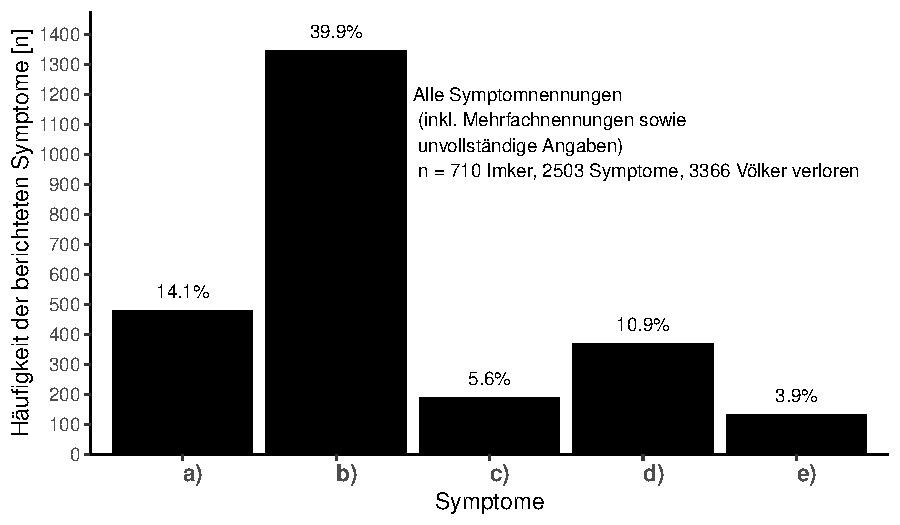
\includegraphics[keepaspectratio,width=0.8\textwidth]{project-U-wintersterblichkeit/figures/plot_symptome}
%  \caption{Häufigkeit der von ImkerInnen berichteten Symptome a) bis e) in Prozent für 2019/20: a) Viele tote Bienen im oder vor dem Volk, b) keine oder nur wenige tote Bienen im oder vor dem Volk, c) tote Bienen in Zellen, kein Futter im Stock, d) tote Bienen in Zellen, aber genug Futter im Stock, e) keines der oben genannten oder unbekannte Symptome.}
%  \label{fig:u:loss:symptome}
%\end{figure}


\subsection{Verteilung der Völkerverluste}

Für die Berechnung wird für jeden einzelnen Imkereibetrieb die Höhe des Gesamtverlustes (d.h. die Summe der toten oder verlorenen Völker und der von Königinnen-Problemen betroffenen Völker) der insgesamt eingewinterten Völker in Prozent berechnet. Insgesamt haben 35,6\% unserer TeilnehmerInnen keine Verluste erlitten. Zwischen >0-20\% haben  38.5\% der ImkerInnen Verluste gemeldet \cref{fig:u:loss:distribution}. Verluste über 20\% haben 25,9\% der TeilnehmerInnen angegeben. Hier sei noch einmal angemerkt, dass die Berechnung der Verlustraten in unserer Analyse auf den jeweiligen Gesamtzahlen basiert und nicht auf Betriebsebene durchgeführt wird.

\begin{figure}[H]
  \centering
  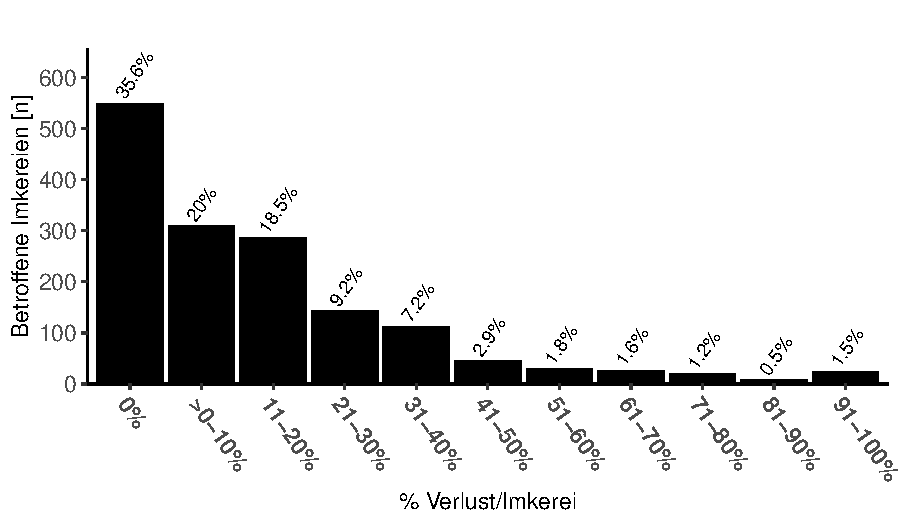
\includegraphics[keepaspectratio,width=0.8\textwidth]{project-U-wintersterblichkeit/figures/plot_overview_loss_dist}
  \caption{Verteilung der Verluste in Prozent pro teilnehmender Imkerei in 10\%-Verlustgruppen, extra angeführt sind TeilnehmerInnen ohne Verluste in der Gruppe \enquote{0\%}.}
  \label{fig:u:loss:distribution}
\end{figure}

\subsection{Risikoanalyse}

In der Risikoanalyse werden die Winterverlustraten verschiedener Gruppen von Betriebsweisen miteinander verglichen. Besteht beispielsweise zwischen zwei Gruppen von Betriebsweisen ein signifikanter Unterschied, kann man daraus Schlussfolgerungen über die Bedeutung dieses Risikofaktors für Winterverluste von Bienenvölkern ziehen. Überlappen die Konfidenzintervalle der Verlustraten von zwei oder mehreren Gruppen nicht, kann die untersuchte Betriebsweise, oder andere damit verknüpfte aber nicht erhobene Faktoren, als signifikanter Einflussfaktor auf die Höhe der Winterverluste betrachtet werden. In weiterer Folge werden die folgenden Faktoren dargestellt:
\ref{ss:seehoehe:U} \nameref{ss:seehoehe:U},
\ref{ss:betriebsgroesse:U} \nameref{ss:betriebsgroesse:U},
\ref{ss:betriebsweise:U} \nameref{ss:betriebsweise:U},
\ref{ss:stand_wander:U} \nameref{ss:stand_wander:U},
\ref{ss:vereinigung:U} \nameref{ss:vereinigung:U},
\ref{ss:wabenhygiene:U} \nameref{ss:wabenhygiene:U},
\ref{ss:trachtangebot:U} \nameref{ss:trachtangebot:U},
\ref{ss:baekempfung_varroa:U} \nameref{ss:baekempfung_varroa:U},
\ref{ss:koeniginnen_verluste:U} \nameref{ss:koeniginnen_verluste:U},
\ref{ss:koeniginnen_probleme:U} \nameref{ss:koeniginnen_probleme:U},
\ref{ss:junge_koeniginnen:U} \nameref{ss:junge_koeniginnen:U},
\ref{ss:verkeuppelte_fluegel:U} \nameref{ss:verkeuppelte_fluegel:U}.


\subsubsection{Seehöhe}
\label{ss:seehoehe:U}

Um den Einfluss der Seehöhe auf die Wintersterblichkeit von Bienenvölkern zu untersuchen, wurden die Winterstandorte bezüglich ihrer Seehöhe in fünf Klassen eingeteilt: 0-200 m, 201-400 m, 401-600 m, 601-800 m, >800 m. Um die Genauigkeit der Auswertung zu erhöhen wurden TeilnehmerInnen die \enquote{Nein} oder \enquote{Unsicher} bei der Fragestellung \enquote{Alle Bienenvölker innerhalb eines \SI{15}{\kilo\meter} Radius} angaben sowie ihre Bienenstände in \enquote{mehr als einem Bezirk} verteilt haben wurden nicht in dieser Risikoanalyse beachtet.
\newline
Im Untersuchungsjahr 2019/20 konnte eine signifikant niedrigere Verlustrate bei der Gruppe „>800 m`` mit \confi{11,6}{95}{10,0}{13,4}
und Gruppe „401-600 m`` mit \confi{11,9}{95}{10,6}{13,3} im Vergleich zu der Gruppe „201-400 m`` mit \confi{15,4}{95}{13,8}{17,3}
festgestellt werden.
\newline
Die zwei restlichen Verlustraten verteilen sich wie folgt: Gruppe „0-200 m`` mit \confi{15,3}{95}{12,0}{19,4} und Gruppe „601-800 m`` mit \confi{13,0}{95}{11,0}{15,3}.

\begin{figure}[H]
  \centering
  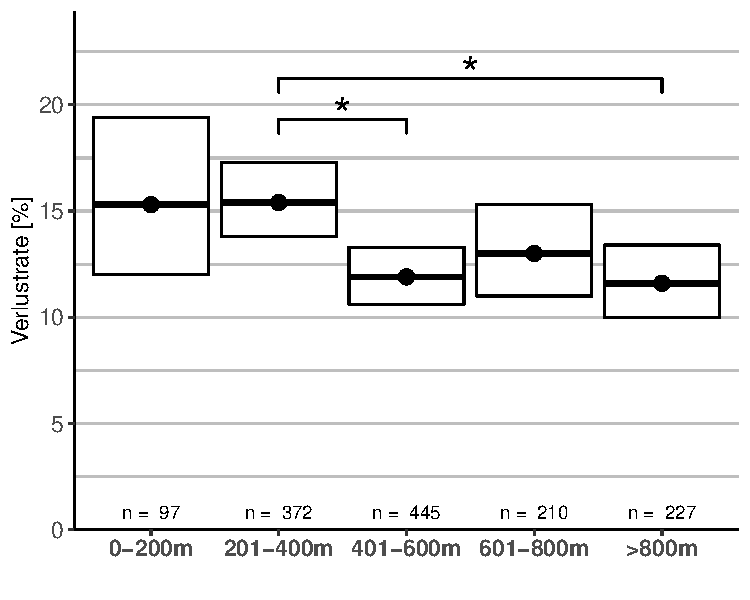
\includegraphics[keepaspectratio,width=0.6\textwidth]{project-U-wintersterblichkeit/figures/plot_elevation}
  \caption{Höhe der Winterverluste 2019/20 in Prozent ($\pm$95\%KI) in Abhängigkeit von der Seehöhe der Winterstandorte. Nicht ausgewertet sind TeilnehmerInnen die \enquote{Nein} oder \enquote{Unsicher} bei Fragestellung \enquote{Alle Bienenvölker innerhalb eines  \SI{15}{\kilo\meter} Radius} Angaben, sowie ihre Bienenvölker in \enquote{mehr als einem Bezirk} aufgestellt haben.}
  \label{fig:u:elevation}
\end{figure}

\subsubsection{Betriebsgröße}
\label{ss:betriebsgroesse:U}

Die Analyse der Erhebung 2019/20 hat gezeigt, dass die Betriebsgröße von Imkereien, wie auch in vergangenen Jahren, einen Risikofaktor für Winterverluste darstellt.
\newline
Es zeigt sich ein signifikante niedrigere Verlustrate für ImkerInnen mit mehr als 50 Völkern (\confi{10,2}{95}{9,2}{11,2}) im Vergleich zu der Gruppe mit 1-50 Völkern mit \confi{14,1}{95}{13,2}{15,0} (\cref{fig:u:factor:operationsize}-A). Wurde diese Aufgliederung zur genaueren Betrachtung in drei Gruppen (Betriebe mit 1 bis 20 Völkern, solche mit 21-50 Völkern und Betriebe mit mehr als 50 Völkern) anstatt zwei unterteilt, zeigten sich 2019/20 signifikant höhere Verluste bei der Gruppe „1-20`` mit \confi{15,1}{95}{13,9}{16,4} und der Gruppe „21-50`` mit \confi{12,9}{95}{11,7}{14,3} im Vergleich zur Gruppe mit über 50 Völkern (\cref{fig:u:factor:operationsize}-B).

\myfig{project-U-wintersterblichkeit/figures/plot_factor_operationsize_combined} % Pfad
  {width=1\textwidth} % Größe Relativ zu Text Breite
  {Höhe der Winterverluste 2019/20 in Prozent ($\pm$95\%KI) in Abhängigkeit von der Betriebsgröße. (A) Einteilung in 1-50 und >50 Völker. (B) Einteilung in 1-20, 21-50 und >50 Völker.} % Text unterhalb der Grafik
  {Optionaler Kurz Titel} % Optional Kurz Überschrift
  {fig:u:factor:operationsize} % Label zum Verweisen im Text

\subsubsection{Betriebsweise}
\label{ss:betriebsweise:U}

Seit 2016/17 werden die ImkerInnen, auch auf eigenen Wunsch, zu weiteren Details ihrer Betriebsweise befragt. Dabei konnten Angaben zu den Beuten gemacht und festgehalten werden, ob der Betrieb eine zertifizierte Bio-Imkerei ist, eine Wanderimkerei betreibt, Bienen auf Varroa-Toleranz züchtet, Fremdwachs zukauft oder neu seit 2019/20 ob schwache (weiselrichtige) Völker vor dem Winter zusammegelegt wurden. Über die Hälfte der TeilnehmerInnen haben angegeben einen offenen Gitterboden in ihren Beuten im Winter zu verwenden und fast 50\% haben Wachs von außerhalb des Betriebes zugekauft. Wie auch in der vorjährigen Befragung gab nur ein kleiner Anteil an Betrieben (7,8\%) an, Naturwabenbau ohne Mittelwand zu verwenden. Zertifizierte Bio-Imkereien waren mit 183 Betrieben in der Befragung vertreten. Einen Überblick über die Häufigkeit der verschiedenen Betriebsweisen (Angaben „Ja``, „Nein``, „Unsicher``, „keine Angaben``) bietet die \cref{fig:u:operational:hist}. 
\newline
\cref{fig:u:operational:loss} zeigt den Einfluss der verschiedenen Betriebsweisen auf die Winterverlustraten. In diesem Untersuchungsjahr konnte eine signifikante niedrigere Verlustrate bei TeilnehmerInnen mit Völkern aus \enquote{Zucht aus Varroa-Toleranz} mit \confi{10,3}{95}{8,5}{12,4} im Gegensatz zur Gruppe \enquote{Unsicher} mit \confi{16,7}{95}{12,7}{21,5} gezeigt werden. Kein statistischer Unterschied war zur Gruppe \enquote{Nein} mit einer Verlustrate von \confi{12,7}{95}{12,0}{13,6} (\cref{fig:u:operational:loss}-C) zu erkennen. TeilnehmerInnen die Fremdwachs eingesetzt haben zeigten eine signifikante höhere Verlustrate mit \confi{14,8}{95}{13,4}{16,3} im Gegensatz zu Imkereibetrieben mit eigenen Wachskreislauf (\confi{11,7}{95}{10,9}{12,6}) (\cref{fig:u:operational:loss}-G). Es konnte auch ein signifikanter Unterschied festgestellt werden bei der Frage ob \enquote{Kleine Brutzellen (5,1 mm oder weniger)} verwendet wurden. Hier zeigt sich eine signifikante niedrigere Verlustrate für die Gruppe \enquote{Ja} mit \confi{6,8}{95}{4,9}{9,4} im Gegensatz zu den anderen zwei Gruppen (Nein - \confi{12,6}{95}{11,8}{13,4}, Unsicher - \confi{16,6}{95}{12,7}{21,4}) (\cref{fig:u:operational:loss}-I).
\newline
Kein statistisch signifikanter Unterschied konnte festgestellt werden zwischen Bio-Imkereien \confi{11,3}{95}{10,1}{12,6} und nicht zertifizierten ImkerInnen \confi{12,5}{95}{11,7}{13,4}. Auch kein Unterschied konnte bei der Frage \enquote{Naturwabenbau} beobachtet werden (Ja - \confi{12,6}{95}{10,3}{15,3}, Nein - \confi{12,6}{95}{11,8}{13,4}, Unsicher - \confi{10,6}{95}{7,3}{15,1}). Die Fragen zur Bauart des Bienenstockes hatten in unserer Untersuchung auch keinen Einfluss: \enquote{Kunststoff-Beuten} (Ja - \confi{12,2}{95}{10,2}{14,5}, Nein - \confi{12,5}{95}{11,7}{13,3}); \enquote{Isolierte Beuten im Winter} (Ja - \confi{13,6}{95}{12,0}{15,4}, Nein - \confi{12,6}{95}{11,8}{13,5}, Unsicher - \confi{15,2}{95}{10,2}{22,0}) und \enquote{Offener Gitterboden im Winter} (Ja - \confi{12,9}{95}{12,0}{14,0}, Nein - \confi{12,0}{95}{11,0}{13,1}) (\cref{fig:u:operational:loss}-A,D,E,F,H).

\subsubsubsection{Stand- versus Wanderimkereien}
\label{ss:stand_wander:U}

Für den Winter 2019/20 wurde untersucht, ob sich Wanderimkerei auf die Wintersterblichkeit auswirkt. Die an unserer Studie teilnehmenden ImkerInnen wurden gefragt, ob sie ihre Bienen zu Trachtquellen oder Bestäubungseinsätzen transportieren (Verbringungen im Zuge der Zucht oder Ablegerbildung sind damit exkludiert).
\newline
Es konnte eine signifikante geringere Verlustrate bei Wanderimkereien (\confi{10,5}{95}{9,4}{11,7}) im Vergleich zu Standimkereien \confi{13,8}{95}{12,9}{14,7} festgestellt werden (\cref{fig:u:operational:loss}-B). 

\subsubsubsection{Vereinigung von Völkern}
\label{ss:vereinigung:U}

Neu in der Umfrage 2019/20 ist die Frage ob vor dem Winter bereits schwache (aber weiselrichtige) Völker vereinigt wurden. Insgesamt gaben 13,8\% der TeilnehmerInnen an Völker bereits vor dem Winter zu vereinigen. Zur Winterverlustrate zeigt sich hier kein statistischer Unterschied zwischen den Gruppen (Ja - \confi{12,7}{95}{11,1}{14,4}, Nein - \confi{12,1}{95}{11,3}{13}, Unsicher - \confi{17,8}{95}{11,5}{26,5}) (\cref{fig:u:operational:loss}-J).

\begin{figure}[H]
  \centering
  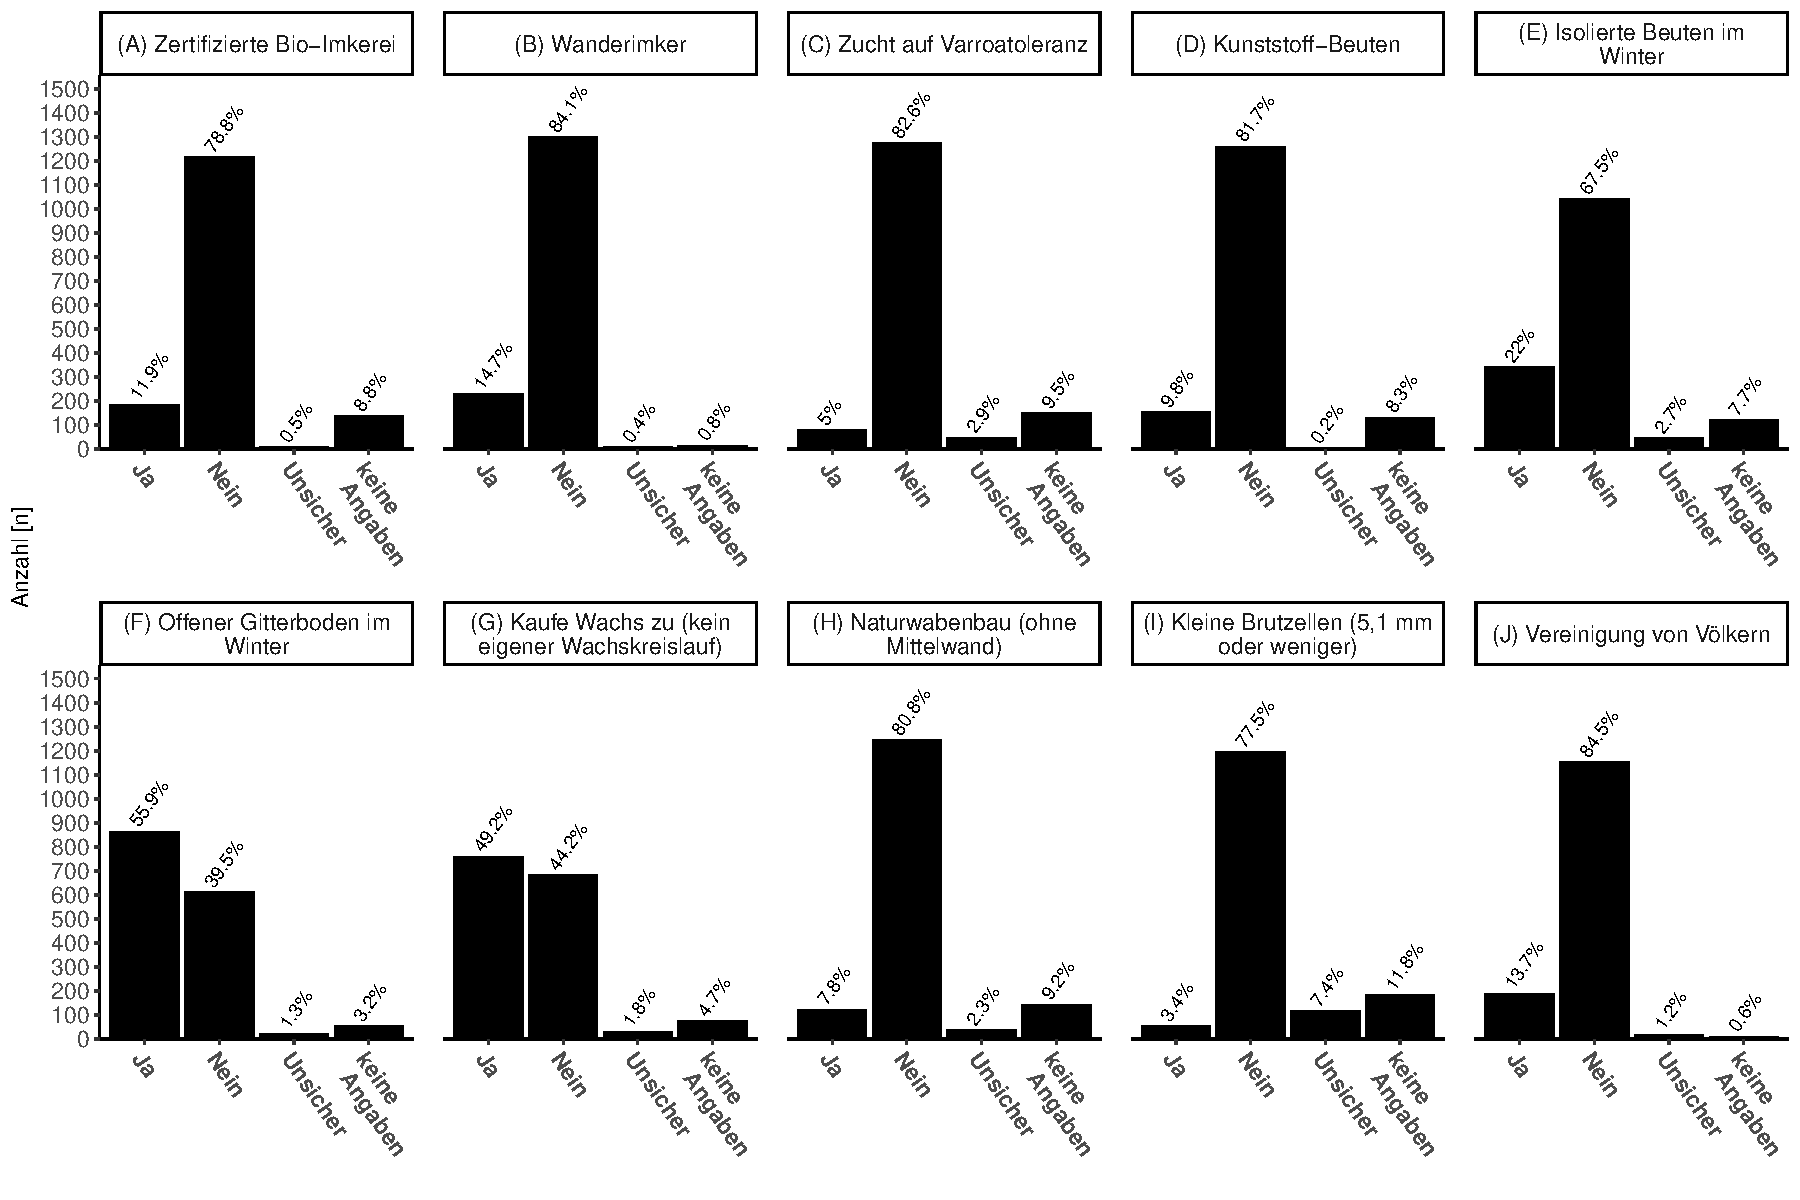
\includegraphics[keepaspectratio,width=1\textwidth]{project-U-wintersterblichkeit/figures/plot_operational_hist}
  \caption{Häufigkeit der Betriebsweisen 2019/20 in unserer Umfrage inklusive Angabe in Prozent.}
  \label{fig:u:operational:hist}
\end{figure}

\begin{figure}[H]
  \centering
  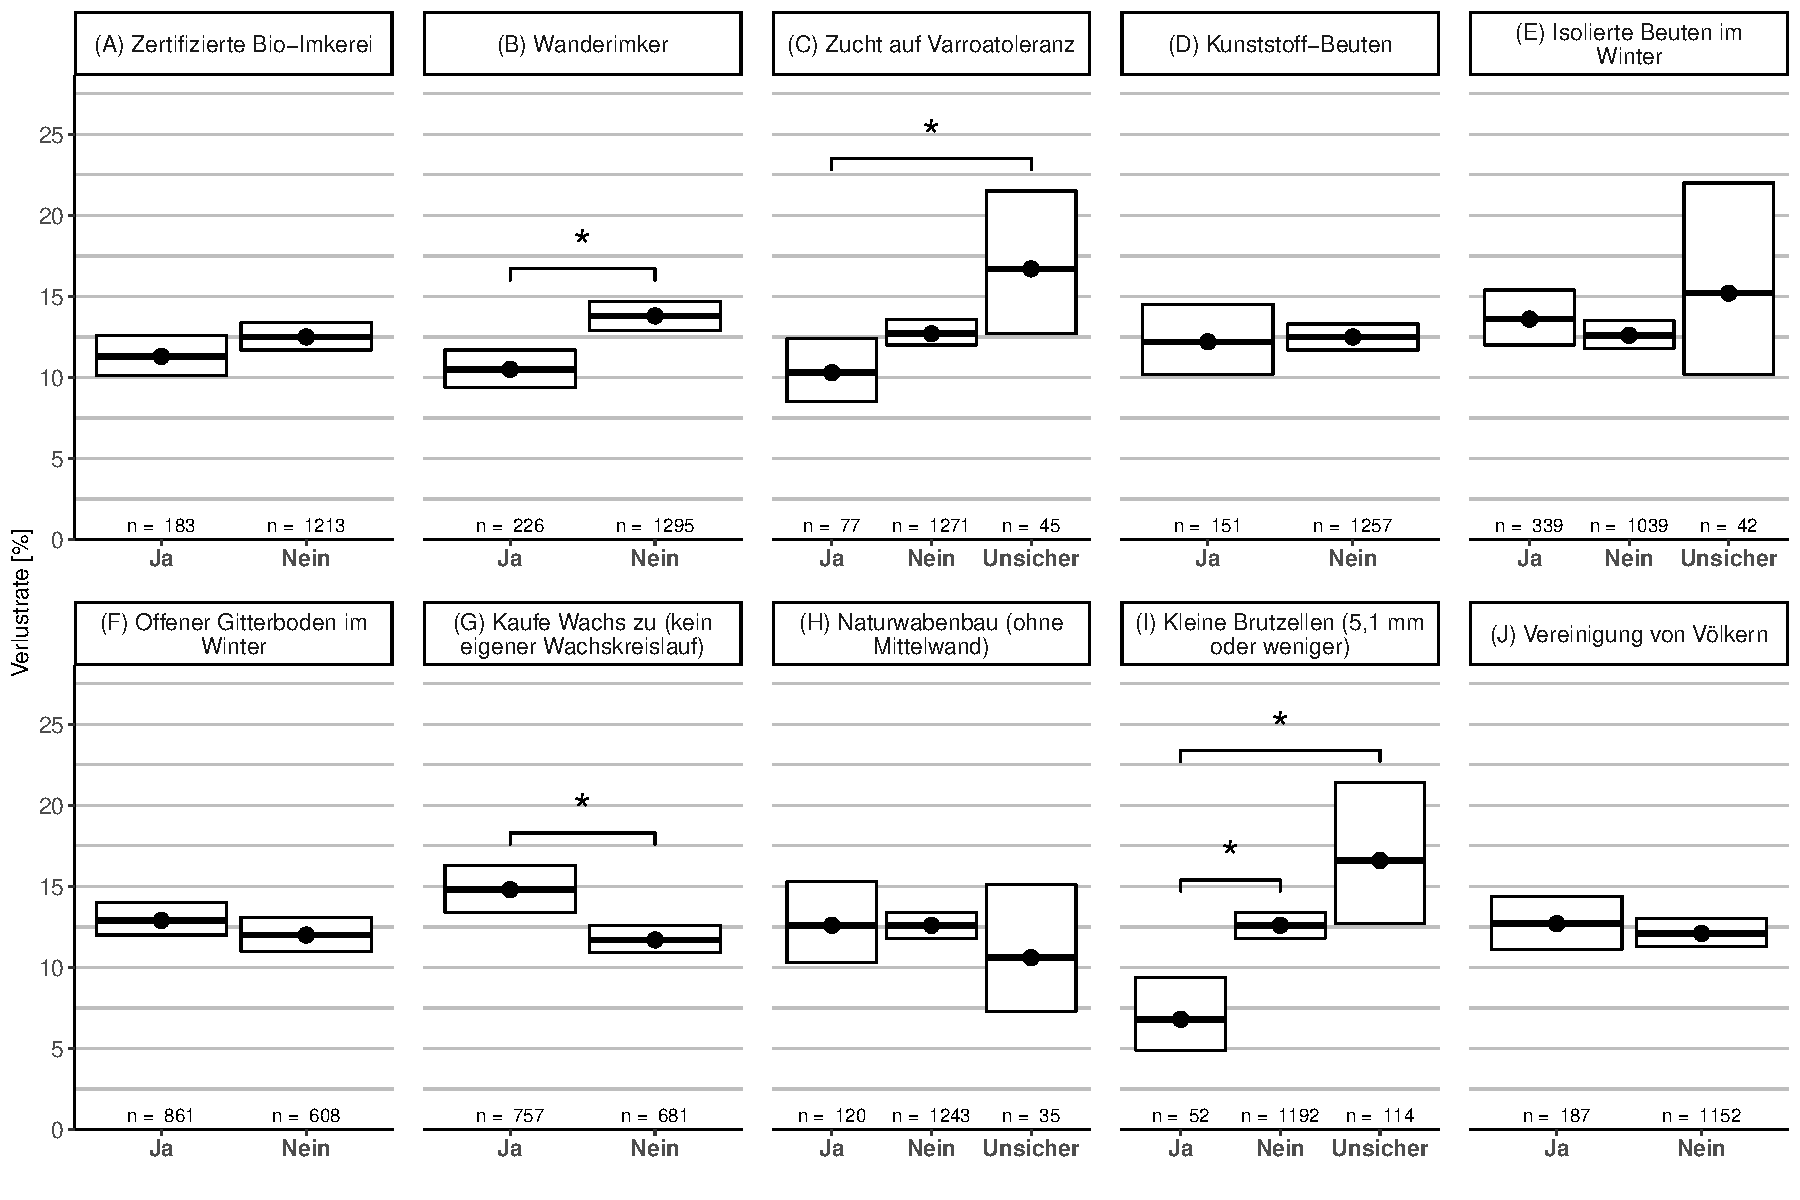
\includegraphics[keepaspectratio,width=1\textwidth]{project-U-wintersterblichkeit/figures/plot_operational_loss}
  \caption{Höhe der Winterverluste 2019/20 in Prozent ($\pm$95\%KI) in Abhängigkeit von der Betriebsweise der TeilnehmerInnen. Die Gruppe mit der Angabe\enquote{Unsicher} wurde nicht ausgewertet wenn \sample{<30}.}
  \label{fig:u:operational:loss}
\end{figure}


\subsubsection{Wabenhygiene}
\label{ss:wabenhygiene:U}

Wabenhygiene in Form von Erneuerung alter Brutwaben kann einen positiven Einfluss auf die Gesundheit der Bienen haben und möglicherweise auch das Überleben der Bienen im Winter beeinflussen. Die ImkerInnen wurden gefragt, welchen Anteil ihrer Brutwaben (in Prozent Klassen) sie erneuert haben. In diesem Jahr konnte kein statistischer Unterschied der Verlustraten zwischen den Gruppen festgestellt werden: Keine Brutwaben erneuert - \confi{14,8}{95}{7,1}{28,4}; Gruppe 1-30\% - \confi{14,2}{95}{12,5}{16,0}; Gruppe 31-50\% - \confi{11,4}{95}{10,4}{12,5} und die Gruppe mit den meisten Erneuerung 51-100\% mit \confi{12,3}{95}{11,2}{13,5}. Die Gruppe der TeilnehmerInnen die zu dieser Frage \enquote{keine Angaben} gemacht hatten zeigt eine Verlustrate von \confi{16,5}{95}{11,4}{23,3} (\cref{fig:u:factor:frames}).

\myfig{project-U-wintersterblichkeit/figures/plot_factor_frames} % Pfad
{width=0.6\textwidth} % Größe Relativ zu Text Breite
{Höhe der Winterverluste von 2019/20 in Abhängigkeit vom Anteil der im Einwinterungsjahr erneuerten Brutwaben in Prozentgruppen ($\pm $95\%KI).} % Text unterhalb der Grafik
{Optionaler Kurz Titel} % Optional Kurz Überschrift
{fig:u:factor:frames} % Label zum Verweisen im Text

\subsubsection{Trachtangebot}
\label{ss:trachtangebot:U}

Die teilnehmenden ImkerInnen wurden nach spezifischen Trachtquellen gefragt, die von ihren Bienen beflogen wurden, um mögliche Risikotrachtquellen zu bestimmen. Zur Auswahl standen 2019/20: Raps (\textit{Brassica napus}), Mais (\textit{Zea mays}), Sonnenblume (\textit{Helianthus annuus}), spätblühende Zwischenfrüchte, Waldtracht sowie Waldtracht mit Melezitose.
\newline
TeilnehmerInnen die eine Raps Tracht hatten zeigten statistisch signifikante höhere Verlustraten (Ja - \confi{13,8}{95}{12,2}{15,5}; Nein - \confi{11,5}{95}{10,7}{12,4}; $\chi^{2}$=20,9, \textit{p}<0,05) (\cref{fig:u:factor:yield}-A). Auch ImkerInnen deren Bienen Mais beflogen zeigten signifikante höhere Verluste (Ja - \confi{17,7}{95}{14,8}{21,0}; Nein - \confi{11,6}{95}{10,8}{12,5}) (\cref{fig:u:factor:yield}-B).
\newline
Ein positiver Effekt konnte bei der Waldtracht festgestellt werden, hier zeigte sich eine signifikant geringere Verlusterate wenn eine Tracht vorhanden war (Ja - \confi{11,4}{95}{10,5}{12,3}; Nein - \confi{14,4}{95}{12,8}{16,2}) (\cref{fig:u:factor:yield}-E).
\newline
Kein statistischer Unterschied konnte bei den anderen in der Umfrage angeführten Trachtquellen festgestellt werden: Sonnenblume (Ja - \confi{14,0}{95}{12,2}{16,0}; Nein - \confi{12,0}{95}{11,1}{12,9}); Spätblüher (Ja - \confi{12,6}{95}{11,6}{13,8}; Nein - \confi{12,6}{95}{11,2}{14,1}) und auch nicht bei Waldtracht mit Melezitose (Ja - \confi{11,6}{95}{10,7}{12,6}; Nein - \confi{13,5}{95}{12,3}{14,8}) (\cref{fig:u:factor:yield}-C,D,F).
\newline
Zur groben Feststellung der Trachtgebiete wurde anhand der Haupt-Überwinterungsstandorte (ohne WanderimkerInnen) eine Karte der betroffenen ImkerInnen aufgezeichnet, welche im Anhang angeführt ist, siehe \cref{fig:u:factor:yield_map}.

\myfig{project-U-wintersterblichkeit/figures/plot_factor_yield} % Pfad
{width=1\textwidth} % Größe Relativ zu Text Breite
{Höhe der Winterverluste von 2019/20 in Abhängigkeit vom Vorhandensein spezifischer Trachtpflanzen in Prozent ($\pm$95\%KI); n=~Anzahl der Betriebe inkl. Wanderimkereien.} % Text unterhalb der Grafik
{Optionaler Kurz Titel} % Optional Kurz Überschrift
{fig:u:factor:yield} % Label zum Verweisen im Text

\subsubsection{Bekämpfung der Varroamilbe}
\label{ss:baekempfung_varroa:U}

Ein wichtiger Teil der Untersuchung sind Erhebungen über die Behandlungsmethoden gegen die Varroamilbe und deren Auswirkung auf die Winterverluste. \cref{fig:u:behandlungsmethoden} zeigt die am Fragebogen zur Auswahl gestellten Behandlungsmethoden. Dabei wird aus Gründen der internationalen Vergleichbarkeit, der von COLOSS erarbeitete Katalog von möglichen Bekämpfungsmethoden verwendet. Nachfolgend wird zuerst die Häufigkeit der verwendeten Methoden dargestellt. Anschließend wurden die einzelnen Methoden im Hinblick auf ihren Einfluss auf die Winterverlustrate betrachtet. Für die detaillierte Risikoanalyse wurden nur jene Behandlungsmethoden berücksichtigt, von denen auch genügend Datensätze vorhanden waren, um eine valide Aussage treffen zu können. Bei der Befragung mittels dem verkürzten Zeitschriftfragebogen wurden keine Details zur Behandlung abgefragt.

\myfig{project-U-wintersterblichkeit/figures/img_behandlungen.png} % Pfad
{width=0.8\textwidth} % Größe Relativ zu Text Breite
{Im Fragebogen zur Auswahl stehende Behandlungsmethoden gegen die Varroamilbe.} % Text unterhalb der Grafik
{Optionaler Kurz Titel} % Optional Kurz Überschrift
{fig:u:behandlungsmethoden} % Label zum Verweisen im Text

91\% der Imkereien bestimmten in mindestens einem Monat des abgefragten Zeitraums den Varroabefall ihrer Völker (zum Beispiel natürlicher Milbenfall mit Stockwindel oder Diagnose mittels Staubzuckermethode) (\cref{tab:u:varroakontrolle}). 
\newline
\cref{tab:u:behandlungsmethoden} zeigt die durchgeführten Methoden der Varroabekämpfung von allen Imkereien, die uns Daten im Untersuchungszeitraum von 2019/20 zur Verfügunggestellt haben.
\newline
Eine der häufigsten Methoden zur Varroabekämpfung ist die Drohnenbrutentnahme, welche von 54,3\% der ImkerInnen in zumindest einem Monat durchgeführt wurde. Danach folgten, nach Häufigkeit der Anwendung, Bekämpfungsmaßnahmen mit organischen Säuren (Ameisensäure Kurzzeit oder Langzeit, unterschiedliche Anwendungsformen der Oxalsäure). Insgesamt 74,8\% der Imkereien in Österreich führten eine Ameisensäurebehandlung durch (Kurzzeit und/oder Langzeit, wobei Langzeitbehandlungen mit 49,1\% in der Imkerschaft etwas häufiger angewandt werden). Von den unterschiedlichen Anwendungen der Oxalsäure, wird die Verdampfung von 51,8\% aller Imkereien angewandt, das Träufeln oder Sprühen von 35,9\% und das Träufeln von Oxalsäureprodukten mit weiteren Inhaltsstoffen (Hiveclean/Bienenwohl/Varromed) von 26,9\% der Imkereien. Die Kombinationsanwendung der beiden organischen Säuren (Ameisensäure kurz oder lang, sowie eine Restentmilbung mit Oxalsäure) wird von 69,3\% der österreichischen Imkereien angewandt. Thymol, egal ob in alleiniger Anwendung oder in Kombination mit anderen Methoden, wurde von 7,7\% der Imkereien als Methode zur Bekämpfung der Varroamilbe verwendet. Biotechnische Methoden abseits der Drohnenbrutentnahme oder Hyperthermie wurden von 25,7\% der Imkereien angewandt, dazu zählen etwa die Fangwabe, die Bannwabe oder die komplette Arbeiterinnen-Brutentnahme. Hyperthermie (=Hitzebehandlung) oder Milchsäure wurden von 4,6\% beziehungsweise 3,5\% der Imkereien angewandt. Synthetische Acarizide zur Bekämpfung der Varroamilbe wurden nur in einem geringen Ausmaß genannt (2,5\%), wobei am häufigsten Amitraz (0,6\%) (Streifen oder Verdampfen) genannt wurde.

\begin{table}[H]
    \centering
    \caption{Anzahl (Prozent) der Imkereien, welche eine Kontrolle der Varroamilbe in zumindest einem Monat durchgeführt haben.}
    \label{tab:u:varroakontrolle}
    \begin{tabular}{l|*{2}{rr|}rr}
        %\hline
            \multicolumn{1}{c}{} & 
            \multicolumn{2}{c|}{Ja} & 
            \multicolumn{2}{c|}{Nein} &
            \multicolumn{2}{c}{keine Angaben} \\ 
        \cline{2-7}
            \multicolumn{1}{c}{} & 
            \makecell{\textit{n}} & \makecell{{\%}} & \makecell{\textit{n}} & \makecell{{\%}} & \makecell{\textit{n}} & \makecell{{\%}} \\
        \hline
        \makecell[l]{Bestimmung Varroabefall \\ (Milbenfall o. ä. Methode)} 
        & 1309 & 91,0\% & 76 & 5,3\% & 54 & 3,8\% \\
        \hline
    \end{tabular}
\end{table}



\begin{table}[H]
    \centering
    \caption{Anzahl (Prozent) der Imkereien, welche die genannte Methode zur Bekämpfung der Varroamilbe in zumindest einem Monat angewendet haben.}
    \label{tab:u:behandlungsmethoden}
    \begin{tabular}{l|*{1}{rr|}rr}
        \toprule            \multirow{2}{*}{\makecell{Behandlungsmethode}} & 
            \multicolumn{2}{c|}{Ja} & 
            \multicolumn{2}{c}{Nein} \\ 
        \cline{2-5}
            & \makecell{\textit{n}} & \makecell{{\%}} & \makecell{\textit{n}} & \makecell{{\%}} \\
        \midrule
        Drohnenbrutentnahme 
        & 778 & 54,3 & 655 & 45,7 \\

        Hyperthermie
        & 66 & 4,6 & 1367 & 95,4 \\

        Andere biotechnische Methode$^1$
        & 368 & 25,7 & 1065 & 74,3 \\

        Ameisensäure KB$^2$ (inkl. MAQS)
        & 538 & 37,5 & 895 & 62,5 \\

        Ameisensäure LB$^2$
        & 703 & 49,1 & 730 & 50,9 \\

        Milchsäure 
        & 50 & 3,5 & 1383 & 96,5 \\

        Oxalsäure Träufeln (oder Sprühen) 
        & 514 & 35,9 & 919 & 64,1 \\

        Oxalsäure Verdampfen
        & 742 & 51,8 & 691 & 48,2 \\

        Hiveclean/Bienenwohl/Varromed
        & 386 & 26,9 & 1047 & 73,1 \\

        Thymol (Apiguard, Apilife VAR, Thymovar)
        & 111 & 7,7 & 1322 & 92,3 \\

        Tau-fluvalinat (Apistan)
        & 3 & 0,2 & 1430 & 99,8 \\

        Flumethrin (Bayvarol)
        & 7 & 0,5 & 1426 & 99,5 \\

        Amitraz (in Streifen, Apivar, Apitraz)
        & 9 & 0,6 & 1424 & 99,4 \\

        Amitraz (Verdampfen) 
        & 9 & 0,6 & 1424 & 99,4 \\

        Coumaphos (Perizin)
        & 0 & 0,0 & 1433 & 100,0 \\

        Coumaphos (Checkmite+)
        & 0 & 0,0 & 1433 & 100,0 \\

        Anderes chemisches Produkt
        & 8 & 0,6 & 1425 & 99,4 \\

        Andere Methode
        & 22 & 1,5 & 1411 & 98,5 \\

        \midrule 
        \textbf{Kombination} &  &  &  &  \\
        \midrule 
        
        \makecell[l]{Ameisensäure (KB oder LB$^2$)} 
        & 1072 & 74,8 & 361 & 25,2 \\
        \makecell[l]{Ameisensäure (KB oder LB$^2$) und \\ Oxalsäurebehandlung$^3$} 
        &  993 & 69,3 & 440 & 30,7 \\
        \bottomrule
        \multicolumn{5}{l}{
            \shortstack[l]{
            $^1$ Beispiel: Fangwabe, Bannwabe, totale Brutentnahme etc.
            \\
            $^2$ KB = Kurzzeitbehandlung, LB = Langzeitbehandlung
            \\
            $^3$ Träufeln oder Sprühen oder Verdampfen oder \\ Hiveclean/Bienenwohl/Varromed
            }
        }
    \end{tabular}
\end{table}

\subsubsubsection{Bestimmung des Varroabefalls}

Um herauszufinden, ob die Bestimmung des Varroabefalls und möglicherweise daraus resultierende Handlungen einen Einfluss auf die Wintersterblichkeit haben könnte, wurden die ImkerInnen gefragt, ob sie den Varroabefall mit einer Methode bestimmt hatten oder nicht. Bei ImkerInnen, die den Varroabefall bestimmt hatten, lag die Verlustrate bei \confi{12,3}{95}{11,6}{13,1} und bei jenen die keine Bestimmung des Varroabefalls durchgeführt hatten bei \confi{12,4}{95}{9,8}{15,5} (\cref{fig:u:treatment:varroa:checked}).

\myfig{project-U-wintersterblichkeit/figures/plot_treatment_varroa_checked} % Pfad
{width=0.6\textwidth} % Größe Relativ zu Text Breite
{Höhe der Winterverluste von 2019/20 in Prozent ($\pm$95\%KI) in Abhängigkeit von einer durchgeführten Abschätzung des Varroabefalls mit nicht näher abgefragten Methoden.} % Text unterhalb der Grafik
{Optionaler Kurz Titel} % Optional Kurz Überschrift
{fig:u:treatment:varroa:checked} % Label zum Verweisen im Text

Auch ein möglicher Effekt der Bestimmungsdauer bzw. Häufigkeit wurde analysiert, das heißt die Anzahl der Monate, in denen die Bestimmung durchgeführt wurde. Die Bestimmungsdauer wurde in drei Klassen unterteilt: Null Monate (keine Bestimmung), Bestimmungszeitraum von einem bis drei Monaten und Bestimmungszeitraum über mehr als drei Monate. Es konnte kein statistisch signifikanter Unterschied zwischen der Gruppe die den Varroa-Befall nicht bestimmt hat \confi{12,4}{95}{9,8}{15,5} zu den beiden anderen Gruppen (1-3 Monate: \confi{12,1}{95}{11}{13,3}; >3 Monate: \confi{12,4}{95}{11,3}{13,4}) festgestellt werden (\cref{fig:u:treatment:varroa:grouped}). 
\newline
Analog zu den vorangegangenen Untersuchungsjahren wurden die Häufigkeiten der Varroa-bestimmung für jeden Monat des Zeitraums zwischen April des Einwinterungsjahres und April des Auswinterungsjahres errechnet. Diese sind in \cref{fig:u:treatment:varroa:overview} dargestellt. Die Methode „Varroabestimmung`` wird vorwiegend in den Monaten Juli bis September, von jeweils über 50\% der teilnehmenden Imkereien angewandt.

\myfig{project-U-wintersterblichkeit/figures/plot_treatment_varroa_grouped} % Pfad
{width=0.6\textwidth} % Größe Relativ zu Text Breite
{Höhe der Winterverluste von 2019/20 in Prozent ($\pm$95\%KI) in Abhängigkeit von der Dauer der Bestimmung des Varroabefalls.} % Text unterhalb der Grafik
{Optionaler Kurz Titel} % Optional Kurz Überschrift
{fig:u:treatment:varroa:grouped} % Label zum Verweisen im Text

\myfig{project-U-wintersterblichkeit/figures/plot_treatment_varroa_overview} % Pfad
{width=0.8\textwidth} % Größe Relativ zu Text Breite
{Häufigkeiten der Bestimmung des Varroabefalls 2019/20 vom April des Einwinterungsjahres bis März des Auswinterungsjahres in Prozent (\textit{n} = siehe \cref{tab:u:varroakontrolle}). April-Mai wurde als Frühjahr definiert (blau), Juni-Oktober als Sommer (grün) und November-Jänner als Herbst/Winter (schwarz), Frühjahr des Folgejahres Februar-März (weiß).} % Text unterhalb der Grafik
{Optionaler Kurz Titel} % Optional Kurz Überschrift
{fig:u:treatment:varroa:overview} % Label zum Verweisen im Text

Des Weiteren wurde untersucht, ob der Zeitpunkt (Jahreszeiten Einteilung siehe \cref{fig:u:treatment:varroa:overview}, exklusive Frühjahr Folgejahr) und die Kombination der Bestimmung des Varroabefalls einen Einfluss auf den Überwinterungserfolg hat. \cref{fig:u:treatment:varroa:combination} zeigt die Winterverlustrate der TeilnehmerInnen in den unterschiedlichen Zeitpunkten und deren Kombinationsmöglichkeiten. Innerhalb der Gruppen und auch im Vergleich zu TeilnehmerInnen die keine Kontrolle durchgeführt haben gibt es keine statistischen signifikante Unterschiede. Die kleinste Gruppe war \enquote{Frühling und Winter} mit nur einem/r TeilnehmerIn und wurde nicht in die Auswertung aufgenommen. Die meisten ImkerInnen haben eine Kontrolle im \enquote{Sommer und Winter} durchgeführt, was innerhalb der Personen die eine Kontrolle durchgeführt haben 35,5\% entspricht.

\myfig{project-U-wintersterblichkeit/figures/plot_treatment_varroa_combination} % Pfad
{width=0.8\textwidth} % Größe Relativ zu Text Breite
{Höhe der Winterverluste von 2019/20 in Prozent ($\pm$95\%KI) in Abhängigkeit von der Bestimmung des Varroa-Befallsgrades im jeweiligen Jahreszeiten. Imker die \enquote{Unsicher} bei Varroa Kontrolle angegeben haben wurden aus dieser Analyse ausgenommen. Einzelne Monate zusammengefasst siehe \cref{fig:u:treatment:varroa:overview}, exkl. Frühjahr Folgejahr.} % Text unterhalb der Grafik
{Optionaler Kurz Titel} % Optional Kurz Überschrift
{fig:u:treatment:varroa:combination} % Label zum Verweisen im Text

\subsubsubsection{Zeitpunkt und Häufigkeit der Anwendungen}

Die TeilnehmerInnen wurden zu ihren verwendeten Methoden zur Bekämpfung der Varroamilbe befragt. Aus den erhaltenen Antworten haben wir die Häufigkeiten, mit der die jeweiligen Methoden in den einzelnen Monaten des Untersuchungsjahres angewendet wurden, bestimmt und in \cref{fig:u:treatment:histogramm} dargestellt.  \\
Die Monate wurden farblich zusammengefasst in Frühjahr, Sommer und Winter zur weiteren Auswertung der Verlustraten. Hierbei wurde April-Mai als Frühjahr definiert (blau), Juni-Oktober als Sommer (grün) und November-Jänner als Herbst/Winter (schwarz). Die Monate Februar, März 2020 (weiß) sind in der folgenden Winter-Verlustanalyse nicht inkludiert.

\begin{figure}[H]
  \centering
  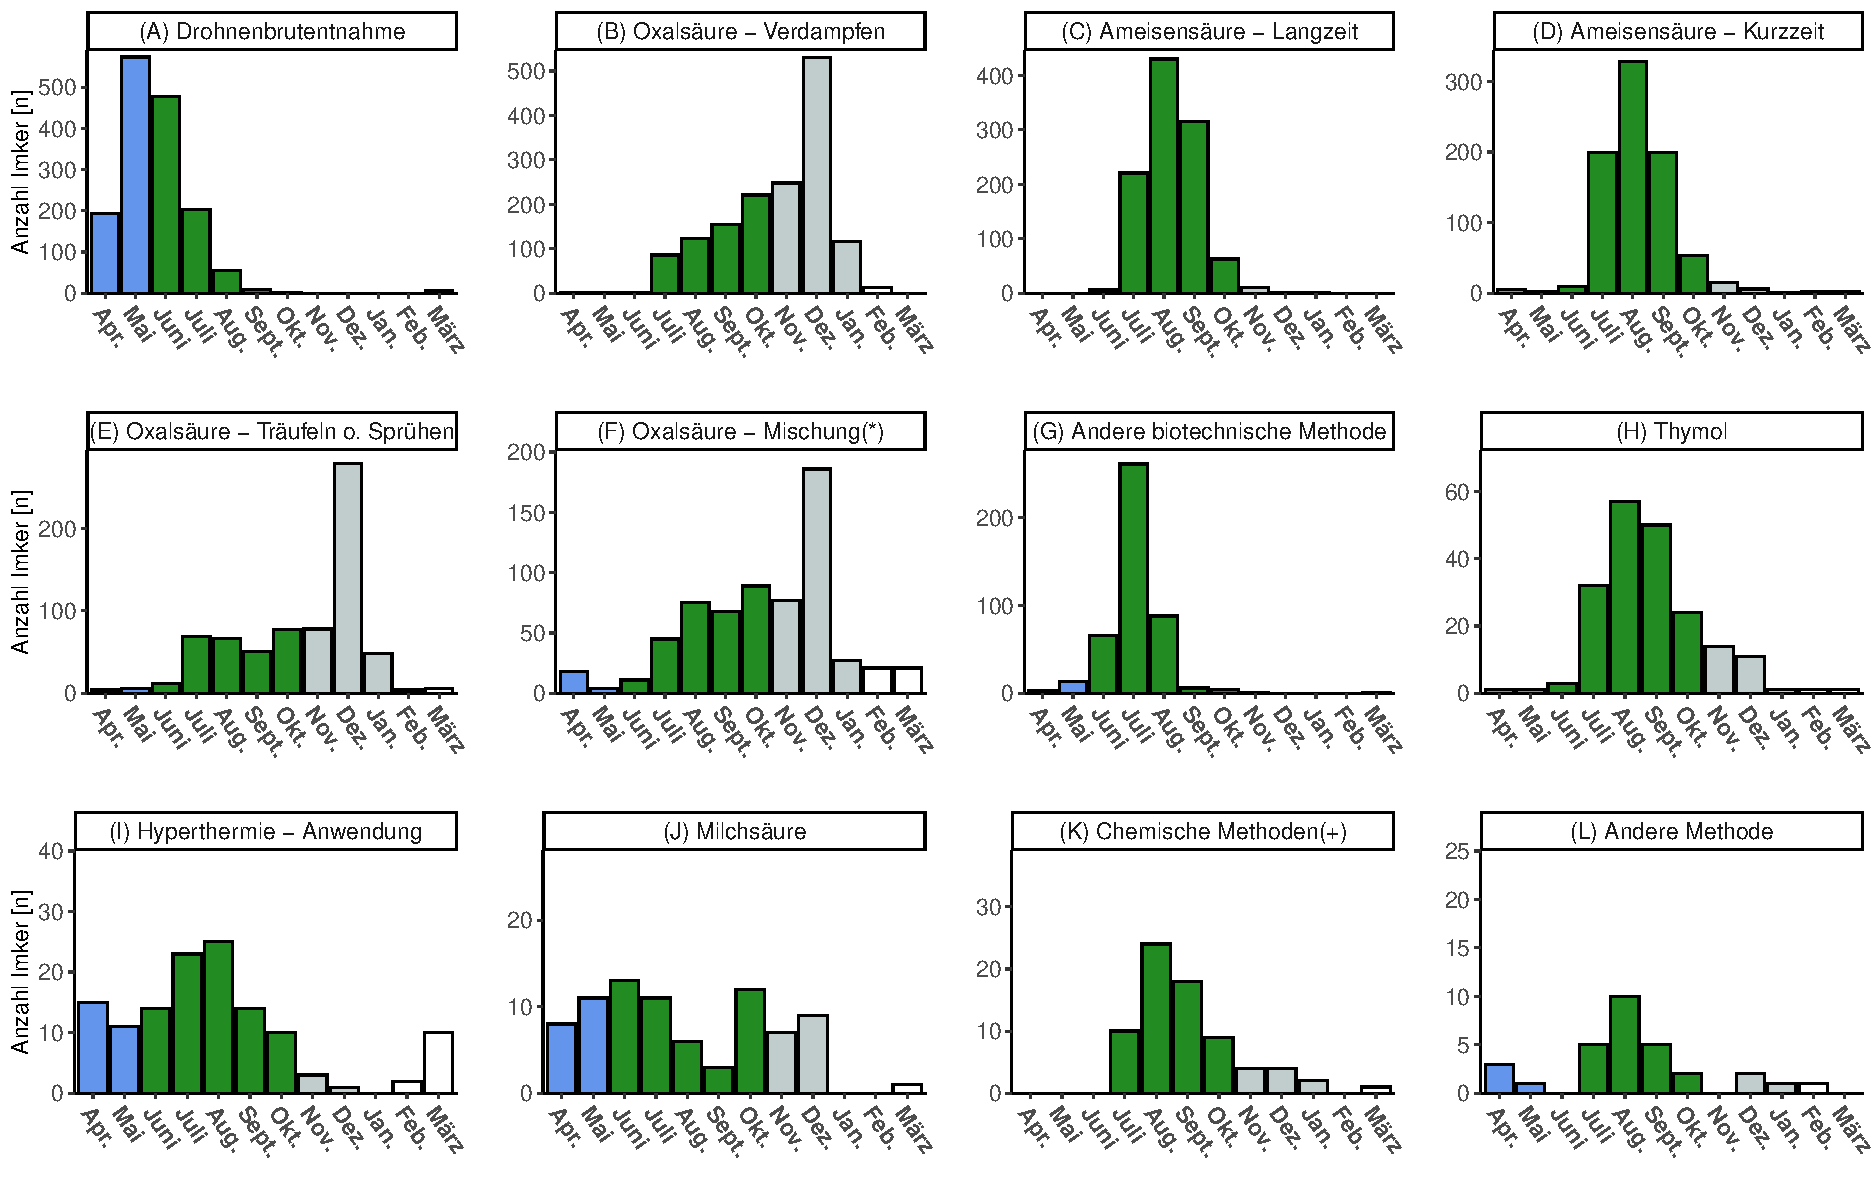
\includegraphics[keepaspectratio,width=1\textwidth]{project-U-wintersterblichkeit/figures/plot_treatment_histogramm}
  \caption{Zusammenfassung der zur Bekämpfung der Varroamilbe angewandten Methoden für das Untersuchungsjahr 2019/20 in den einzelnen Monaten. Y-Axis mit separaten Skalen für die verschiedenen Behandlungsmethoden. April-Mai wurde als Frühjahr definiert (blau), Juni-Oktober als Sommer (grün) und November-Jänner als Herbst/Winter (schwarz). Die Monate Februar, März 2020 (weiß) sind in der folgenden Winter-Verlustanalyse nicht inkludiert. 
  \newline 
  (+) Amitraz (verdampfe und in Streifen, Apivar, Apitraz), Coumaphos (Checkmite+), Coumaphos (Perizin), Flumethin (Bavarol), Tau-fluvalinat (Apistan), Anderes Chemisches Produkt  
  \newline 
  (*) Hiveclean, Bienenwohl, Varromed}
  \label{fig:u:treatment:histogramm}
\end{figure}

\subsubsubsection{Anwendungen in den Jahreszeiten}

Die Verlustrate und statistischen Ergebnissen mit den einzelnen Behandlungsmethoden laut \cref{fig:u:treatment:spring,fig:u:treatment:summer,fig:u:treatment:winter} werden in den folgenden Unterkapiteln näher betrachtet. Mögliche Behandlungen im Frühjahr des Folgejahres (Februar, März) sind nicht inkludiert. Die \enquote{Chemischen Methoden} wurden zusammengefasst wegen der geringen Strichprobenanzahl, siehe \cref{tab:u:behandlungsmethoden}. Sowie \enquote{Oxalsäure - Träufeln o. Sprühen} und \enquote{Oxalsäure - Mischung} werden gemeinsam betrachtet, eine getrennte Analyse der zwei Methoden findet sich im Unterkapitel \ref{sss:mischungox:u} \nameref{sss:mischungox:u}.

\myfig{project-U-wintersterblichkeit/figures/plot_treatment_spring} % Pfad
{width=1\textwidth} % Größe Relativ zu Text Breite
{Höhe der Winterverluste von 2019/20 in Prozent ($\pm$95\%KI) in Abhängigkeit von der Behandlungsmethode. Einzelne Monate sind nach Saison zusammengefasst, siehe \cref{fig:u:treatment:histogramm}.
\newline
(*) Hiveclean, Bienenwohl, Varromed
} % Text unterhalb der Grafik
{Optionaler Kurz Titel} % Optional Kurz Überschrift
{fig:u:treatment:spring} % Label zum Verweisen im Text

\myfig{project-U-wintersterblichkeit/figures/plot_treatment_summer} % Pfad
{width=1\textwidth} % Größe Relativ zu Text Breite
{Höhe der Winterverluste von 2019/20 in Prozent ($\pm$95\%KI) in Abhängigkeit von der Behandlungsmethode. Einzelne Monate sind nach Saison zusammengefasst, siehe \cref{fig:u:treatment:histogramm}.
\newline 
(+) Amitraz (verdampfe und in Streifen, Apivar, Apitraz), Coumaphos (Checkmite+), Coumaphos (Perizin), Flumethin (Bavarol), Tau-fluvalinat (Apistan), Anderes Chemisches Produkt  
\newline
(*) Hiveclean, Bienenwohl, Varromed}
{Optionaler Kurz Titel} % Optional Kurz Überschrift
{fig:u:treatment:summer} % Label zum Verweisen im Text

\myfig{project-U-wintersterblichkeit/figures/plot_treatment_winter} % Pfad
{width=1\textwidth} % Größe Relativ zu Text Breite
{Höhe der Winterverluste von 2019/20 in Prozent ($\pm$95\%KI) in Abhängigkeit von der Behandlungsmethode. Einzelne Monate sind nach Saison zusammengefasst, siehe \cref{fig:u:treatment:histogramm}.
\newline 
(*) Hiveclean, Bienenwohl, Varromed}
{Optionaler Kurz Titel} % Optional Kurz Überschrift
{fig:u:treatment:winter} % Label zum Verweisen im Text

\subsubsubsection{Auswirkungen der Drohnenbrutentnahme auf die Winterverluste}
\label{sss:drohnenbrutentahme:u}

Eine der am häufigsten angewandten Methoden zur Verringerung des Varroabefalls ist die Drohnenbrutentnahme. Von den teilnehmenden Imkereien 2019/20 haben 54,3\% diese Methode in zumindest einem Monat angewandt. TeilnehmerInnen die diese Methode im Frühjahr eingesetzt haben, zeigten statistisch signifikant niedrigere Verlustrate (\confi{11,4}{95}{10,4}{12,4}) als TeilnehmerInnen die diese Methode nicht durchgeführt haben (\confi{13,1}{95}{12,1}{14,1}) ($\chi^{2}$=20,4, \textit{p}<0,05) (\cref{fig:u:treatment:spring}-A). Im Sommer konnte kein Unterschied zwischen den Gruppen festgestellt werden (Ja - \confi{12,3}{95}{11,1}{13,5}; Nein - \confi{12,3}{95}{11,5}{13,3}) (\cref{fig:u:treatment:summer}-A).
\newline
Ob der Zeitpunkt der Entnahme von Drohnenbrut einen Einfluss auf die Winterverlustrate hat, wurde durch eine Gegenüberstellung der Verlustraten für die Jahreszeiten und in Kombination analysiert. In \cref{fig:u:treatment:drone:combination} sind die Ergebnisse grafisch dargestellt. Hier zeigt sich das die meisten TeilnehmerInnen die eine Drohnenbrutentahme durchgeführt haben diese im Frühling und Sommer gemacht haben (\sample{385}, \confi{11,3}{95}{10,1}{12,7}). Es konnte kein statistischer signifikanter Unterschied beim Zeitpunkt in den Verlustraten festgestellt werden (Nur Frühling - \confi{11,4}{95}{9,9}{13,1}; Nur Sommer - \confi{15,2}{95}{12,8}{18}). Auch im Vergleich zur Gruppe die keine Drohnenbrutentahme durchgeführt hat ergibt sich kein statistischer Unterschied (\confi{13,3}{95}{12,2}{14,4}). 

\myfig{project-U-wintersterblichkeit/figures/plot_treatment_drone_combination} % Pfad
{width=0.8\textwidth} % Größe Relativ zu Text Breite
{Höhe der Winterverluste von 2019/20 in Prozent ($\pm$95\%KI) in Abhängigkeit von der Behandlungsmethode \enquote{Dronenbrutentnahme} und Zeitpunkt der Durchführung. Einzelne Monate zusammengefasst siehe \cref{fig:u:treatment:histogramm}.} % Text unterhalb der Grafik
{Optionaler Kurz Titel} % Optional Kurz Überschrift
{fig:u:treatment:drone:combination} % Label zum Verweisen im Text

Zusätzlich wurde die Auswirkung einer mehrfachen Drohnenbrutentnahme auf die Winterverluste untersucht. Das heißt ob die Anzahl der Monate, in denen eine Drohnenbrutentnahme durchgeführt wurde, einen Einfluss auf den Überwinterungserfolg hat. Dazu wurden die Verlustraten der Gruppen „0`` (=keine Behandlung) (\confi{13,3}{95}{12,2}{14,4}), „1-3 Monate`` (\confi{12,1}{95}{11,1}{13,1}) und „>3 Monate`` (\confi{11,5}{95}{8,4}{15,4}) verglichen. Bei dieser Untersuchung konnte kein signifikanter Unterschied aufgrund der Dauer der Behandlung festgestellt werden (\cref{fig:u:treatment:drone:grouped}). 

\myfig{project-U-wintersterblichkeit/figures/plot_treatment_drone_grouped} % Pfad
{width=0.6\textwidth} % Größe Relativ zu Text Breite
{Höhe der Winterverluste von 2019/20 in Prozent ($\pm$95\%KI) in Abhängigkeit von der Dauer der Drohnenbrutentnahme.} % Text unterhalb der Grafik
{Optionaler Kurz Titel} % Optional Kurz Überschrift
{fig:u:treatment:drone:grouped} % Label zum Verweisen im Text


\subsubsubsection{Ameisensäure-Behandlung}

Wir haben bei unseren Analysen zwischen Kurzzeit- und Langzeitbehandlung mit Ameisensäure unterschieden und die daraus resultierenden Verlustraten miteinander verglichen. Es ist zu vermerken, dass bei keiner der Methoden die Konzentration der verwendeten Ameisensäure abgefragt wurde.
\newline
Im Sommer zeigt sich für die Kurzzeitbehandlung kein statistischer Unterschied zwischen den ImkerInnen die diese Behandlung durchgeführt haben und denen, die sie nicht durchgeführt haben (Ja - \confi{12,8}{95}{11,7}{13,9}; Nein - \confi{12}{95}{11,1}{13}) (\cref{fig:u:treatment:summer}-D). Eine Langzeitbehandlung im Sommer führte zu statistisch signifikanten niedrigeren Verlustraten (\confi{11,4}{95}{10,4}{12,5}) im Verlgeich zur Gruppe die keine Langzeitbehandlung durchgeführt hat (\confi{13}{95}{12,1}{14,1}) ($\chi^{2}$=17,9, \textit{p}<0,05) (\cref{fig:u:treatment:summer}-E). In den von uns definierten Monaten im Winter hatte eine Kurzzeitbehandlung mit Ameisensäure eine statistisch signifikante negative Auswirkungen auf die Verlustraten (Ja - \confi{23,6}{95}{13,5}{37,9}; Nein - \confi{12,2}{95}{11,5}{13}) (\cref{fig:u:treatment:winter}-A).
\newline
Betrachtet man ImkerInnen die ausschließlich eine Kurzzeitbehandlung im Sommer durchgeführt haben, zeigen sich potentiell hohe Winterverlustraten (\confi{23,3}{95}{13,8}{36,5}) im Gegensatz zu den Imker die außschließlich eine Langzeitbehandlung im Sommer durchgeführt haben (\confi{15,3}{95}{11,4}{20,4}) \cref{fig:u:combination}.

\subsubsubsection{Oxalsäure}

Während der Wintermonate setzen viele ImkerInnen Oxalsäure zur Bekämpfung der Varroamilbe zur sogenannten Restentmilbung ein. In besonderen Situationen kann eine Anwendung auch in der warmen Jahreszeit erfolgen. Die Anwendung dieser Methode erfordert allerdings, dass die Völker brutfrei sind, da die Oxalsäure nicht in die verdeckelte Brut wirkt oder eine mehrmalige Anwendung in kurzen Abständen.
\newline
Die Oxalsäure kann entweder durch Träufeln oder durch Verdampfen eingesetzt werden. Hiveclean, Bienenwohl und Varromed sind
kommerziell erhältliche Fertigmischungen aus Oxalsäure, Zucker und anderen Stoffen, die ebenfalls geträufelt werden. Es wurde untersucht, ob sich die Winterverlustraten bei ImkerInnen, die eine dieser Methoden eingesetzt haben, von jenen, die diese Methoden nicht angewandt haben, unterscheiden.
\newline
Betriebe die im Frühjahr \enquote{Oxalsäure durch Träufeln o. Sprühen (inkl. Fertigmischungen)} eingesetzt haben, zeigten keine statistisch signifikanten Unterschiede in den Winterverlustraten (Ja - \confi{12,8}{95}{9}{17,8}; Nein - \confi{12,3}{95}{11,6}{13}) (\cref{fig:u:treatment:spring}-C). Auch in den anderen zwei Jahreszeiten zeigte die Methode zwischen Anwendung und nicht Anwendung keinen signifikanten Unterschied: Sommer (Ja - \confi{12,6}{95}{11,3}{14}; Nein - \confi{12,2}{95}{11,4}{13,1}) (\cref{fig:u:treatment:summer}-H); Winter (Ja - \confi{13,1}{95}{12}{14,3}; Nein - \confi{11,8}{95}{10,9}{12,7}) (\cref{fig:u:treatment:winter}-C).
\newline
Die gleiche Auswertung für \enquote{Oxalsäure Verdampfen} zeigt im Sommer keinen signifikanten Unterschied in den Verlustraten (Ja - \confi{11,8}{95}{10,5}{13,3}; Nein - \confi{12,5}{95}{11,7}{13,3}) (\cref{fig:u:treatment:summer}-G). Im Winter zeigt sich eine statistisch signifikante niedrigere Verlustrate für Oxalsäure Verdampfen mit \confi{11,5}{95}{10,6}{12,5} als für TeilnehmerInnen die nicht Verdampft haben mit \confi{13,2}{95}{12,1}{14,3} ($\chi^{2}$=18,3, \textit{p}<0,05) (\cref{fig:u:treatment:winter}-B). Eine ausschließliche Behandlung mit Oxalsäure durch Verdampfung wurde von \sample{39} TeilnehmerInnen durchgeführt und führte zu Verlustraten die im österreichischen Durchschnitt liegen (\confi{13,1}{95}{9,9}{17,2}) (\cref{fig:u:combination}-F).

\subsubsubsection{Hiveclean/Bienenwohl/Varromed}
\label{sss:mischungox:u}

Kommerzielle Oxalsäure-Fertigmischungen mit dem Wirkstoff Oxalsäure (und weiteren Hilfsstoffen) werden für einen guten Behandlungserfolg im brutfreien Volk eingesetzt. Im Untersuchungsjahr 2019/20 setzten 26,9\% aller befragten ImkerInnen eines dieser Produkte zur Bekämpfung der Varroa-Milbe ein. Es konnte kein signifikanter Unterschied in der Verlustrate beobachtet werden, wenn eine Fertigmischung zur Bekämpfung der Varroamilbe verwendet wurde mit \confi{12,9}{95}{11,4}{14,6} oder reine Oxalsäure geträufelt wurde \confi{12,8}{95}{11,5}{14,2}.
Auch wenn beides verwendet wurde (\confi{11,8}{95}{9,3}{14,8}) oder keine der beiden Methoden \confi{11,8}{95}{10,8}{12,9} führte es zu keinem statistisch signifikanten Unterschieden \cref{fig:u:treatment:oxalmix}.

\begin{figure}[H]
  \centering
  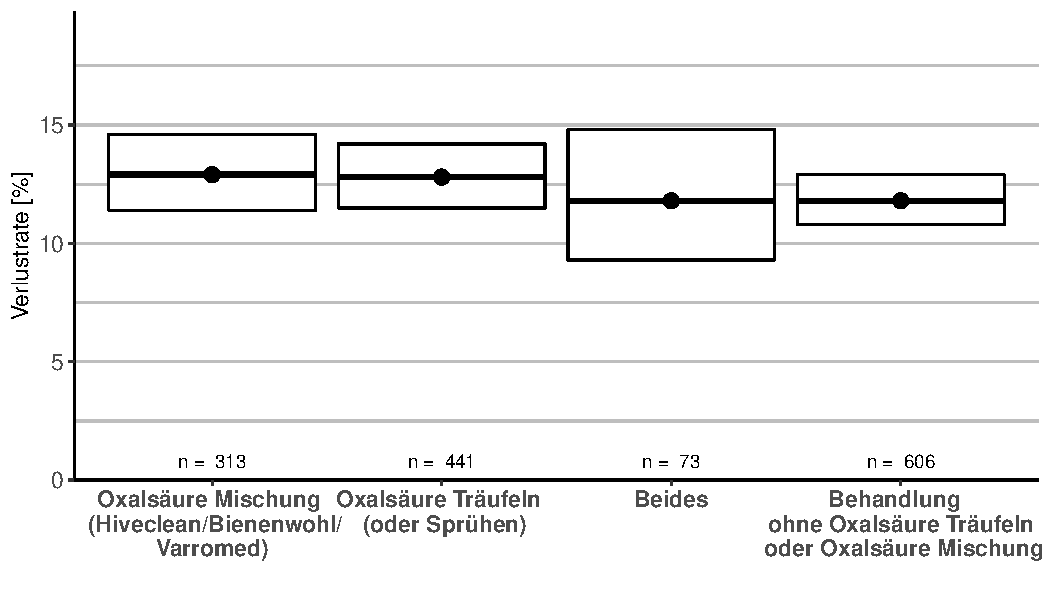
\includegraphics[keepaspectratio,width=0.8\textwidth]{project-U-wintersterblichkeit/figures/plot_treatment_oxalmix}
  \caption{Höhe der Winterverluste von 2019/20 in Prozent ($\pm$95\%KI) in Abhängigkeit von der Varroabekämpfung mit einer Oxalsäure Fertigmischung (Hiveclean, Bienenwohl, Varromed) zu reiner Oxalsäure Lösung, in Kombination und ohne die zwei Methoden.}
  \label{fig:u:treatment:oxalmix}
\end{figure}

\subsubsubsection{Thymol}

Von 7,7\% aller befragten ImkerInnen wurde angegeben, eine Behandlung mit Thymol durchgeführt zu haben. Hierbei zeigt sich für Betriebe die im Sommer Thymol eingesetzt haben statistisch signifikant höhere Verlustrate mit \confi{18,4}{95}{14,9}{22,4} als für die Gruppe die kein Thymol eingesetzt hat \confi{12}{95}{11,3}{12,7} (\cref{fig:u:treatment:summer}-I).
\newline
Betrachtet man die Häufigkeit der Anwendungen in Monaten im Vergleich zu den Winterverlusten, zeigten sich für ImkerInnen mit einmaliger Anwendung statistisch signifikante höhere Verlustraten mit \confi{22,4}{95}{17,4}{28,3} im Verlgeich zu keiner Thymol Behandlung mit \confi{12,3}{95}{11,6}{13}. TeilnehmerInnen die in mehr als einem Monat mit Thymol behandelt haben, zeigen keinen statistischen signifikanten Unterschied \confi{13,9}{95}{9,8}{19,3} (\cref{fig:u:treatment:thymol:grouped}).

\begin{figure}[H]
  \centering
  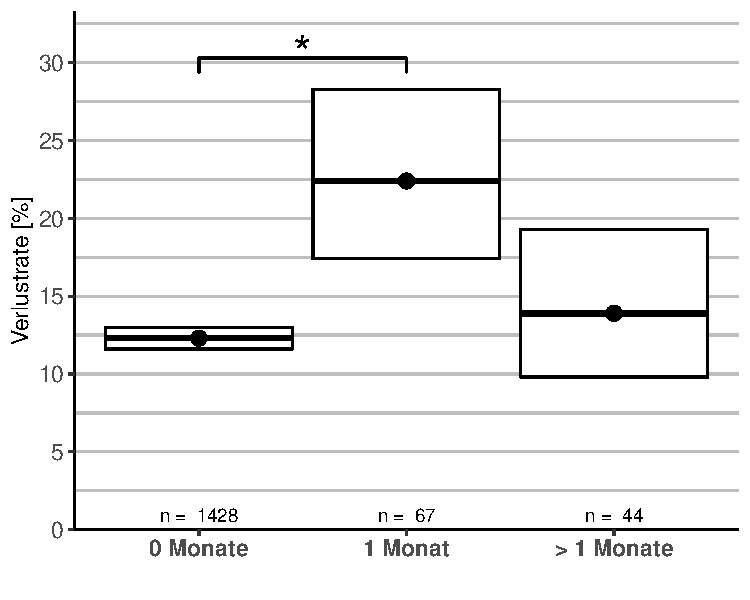
\includegraphics[keepaspectratio,width=0.7\textwidth]{project-U-wintersterblichkeit/figures/plot_treatment_thymol_grouped}
  \caption{Höhe der Winterverluste 2019/20 in Prozent (\(\pm\)95\%KI) in Abhängigkeit von der Häufigkeit der Anwendungen in Monaten von Produkten auf Thymolbasis.}
  \label{fig:u:treatment:thymol:grouped}
\end{figure}

\subsubsubsection{Hyperthermie}

Eine Alternative zur chemischen Behandlung der Völker gegen die Varroamilbe stellt die Hitzebehandlung (=Hyperthermie) dar. Sie beruht auf der unterschiedlichen Wärmetoleranz von Bienen und Milben. 4,6\% der ImkerInnen, die sich an der Erhebung der Winterverluste beteiligt haben, wendeten diese nicht-chemische Behandlung in zumindest einem Monat an. Es wurde nicht zwischen den verschiedenen am Markt erhältlichen Systemen zur Hitzebehandlung unterschieden. Hinsichtlich der Verlustrate fanden wir keine statistischen signifikanten Unterschiede zwischen Imkereien, die mit Hyperthermie behandelt haben und jenen, die nicht damit behandelt haben: Frühjahr (Ja - \confi{12,8}{95}{8,8}{18,2}; Nein - \confi{12,3}{95}{11,6}{13}); Sommer (Ja - \confi{11,9}{95}{9}{15,6}; Nein - \confi{12,3}{95}{11,6}{13,1}) (\cref{fig:u:treatment:spring}, \cref{fig:u:treatment:summer} - B).

\subsubsubsection{Andere biotechnische Methoden (ohne Hyperthermie /  Drohnenbrutentnahme)}

Andere biotechnische Methoden, mit Ausnahme von Hyperthermie und Drohnenbrutentnahme, wurden zusammengefasst abgefragt. 25,7\% der befragten ImkerInnen gaben an eine solche biotechnische Methode angewendet zu haben. Dazu zählen die Verwendung von Fangwaben oder Bannwaben oder die komplette Brutentnahme.
\newline
Im Untersuchungsjahr 2019/20 zeigten sich signifikant niedrigere Verlustraten bei einer Anwendung dieser Methode im Sommer (Ja - \confi{11,2}{95}{10,1}{12,3}; Nein - \confi{13}{95}{12,1}{13,9}; $\chi^{2}$=21,1, \textit{p}<0,05) (\cref{fig:u:treatment:summer} - C). Kombinationen mit anderen Behandlungmittel zeigen Potential für geringe Verlustraten, siehe \ref{sss:kombination:U} \nameref{sss:kombination:U}.

\subsubsubsection{Behandlungskombinationen}
\label{sss:kombination:U}

Die Kombination \cref{fig:u:combination} beinhaltet alle möglichen Kombinationen der Behandlungen nach Jahreszeiten mit mindestens 15 ImkerInnen, ohne Drohnenbrutentnahme. Eine Risikoanalyse zur Drohnenbrutentahme wurde extra angeführt und ausgewertet, siehe \ref{sss:drohnenbrutentahme:u} \nameref{sss:drohnenbrutentahme:u}. Es wurden maximal drei verschiedene Kombinationsmöglichkeiten betrachtet was zu 4535 möglichen Kombinationen geführt hat. Hier wurden statistisch nur die Kombinationen ausgewertet die von mindestens 16 TeilnehmerInnen durchgeführt wurden. Dieser Filter führte zu insgesamt 19 verschiedenen Kombinationen und ihren jeweiligen Verlustraten (\cref{fig:u:combination}, \cref{tab:u:kombinationen}). Hierbei sei bei den Kombinationen mit kleineren Stichproben auf die breiten Konfidenzintervalle hingewiesen.
\newline
Die Kombination mit den meisten TeilnehmerInnen war die Langzeitbehandlung mit Ameisensäure im Sommer gefolgt von einer Oxalsäure Sublimation im Winter (\sample{156}, \confi{10,4}{95}{8,8}{12,3}) (A) bzw. Träufeln im Winter (\sample{95}, \confi{10,9}{95}{8,2}{14,4}) (B). Ein signifikante höhere Verlustrate im Vergleich zum österreichischen Durchschnitt hatten TeilnehmerInnen die nur eine Ameisensäure - Kurzzeitbehadlung im Sommer durchgeführt haben \confi{23,3}{95}{13,8}{36,5} (Q). 
\newline
Biotechnische Maßnahmen im Sommer gefolgt von Oxalsäure im Sommer und Winter zeigt ein Potential für niedrigere Verlustraten gegenüber dem österreichische Durchschnitt ((D) - \confi{10,7}{95}{8,1}{13,9}; (O) - \confi{9,1}{95}{4,3}{18,2}, (P) - \confi{9}{95}{5,6}{14,4}).

\myfig{project-U-wintersterblichkeit/figures/plot_combination_loss} % Pfad
{width=1\textwidth} % Größe Relativ zu Text Breite
{Höhe der Winterverluste von 2019/20 in Prozent ($\pm$95\%KI) in Abhängigkeit von der Behandlungsmethodenkombination und dem Zeitpunkt der Durchführung. Einzelne Monate zusammengefasst siehe \cref{fig:u:treatment:histogramm}. Nur Kombinationen von Methoden mit mindestens 16 TeilnehmerInnen wurden ausgewertet. Die Anzahl der Unterschiedlichen Behandlungsmethoden ist farblich gekennzeichnet (weiß = 1, grau = 2, schwarz = 3). Der Österreichischer Durchschnitt (rote Linie) mit ($\pm$95\%KI) (gestrichelte Linie) ist vertikal eingezeichnet. Abkürzungen der Behandlungsmethoden siehe \cref{tab:u:kombinationen}.} % Text unterhalb der Grafik
{Optionaler Kurz Titel} % Optional Kurz Überschrift
{fig:u:combination} % Label zum Verweisen im Text

\newpage
\begin{landscape}

\begin{table}[H]
  \centering
  \caption{Verlustraten und Stichprobenanzahl der Kombinationen. W = Winter, S = Sommer, Einzelne Monate sind nach Saison zusammengefasst, siehe \cref{fig:u:treatment:histogramm}.}
  \scriptsize
  \setlength{\tabcolsep}{0.5em} % for the horizontal padding
  \label{tab:u:kombinationen}
  \begin{tabular}{l|*{6}{l}|rr}
  \toprule
    \multicolumn{1}{c|}{Abkürzung} & 
    \multicolumn{6}{c|}{Methode} & 
    \multicolumn{1}{c}{\textit{n}} &
    \multicolumn{1}{c}{Verlust (95\% CI)}
    \\
    \midrule
    (A) S-AS-LZ \& W-Ox-Träu. & S & Ameisensäure - Langzeit & W & Oxalsäure - träufeln & & & 138 & 10,1 (8,2-12,5) \\
    (B) S-AS-LZ \& W-Ox-Sub.  & S & Ameisensäure - Langzeit & W & Oxalsäure - sub.     & & & 88  & 11,1 (8,7-14) \\
    (C) S-AS-KZ \& W-Ox-Träu. & S & Ameisensäure - Kurzzeit & W & Oxalsäure - träufeln & & & 61  & 12,1 (9,4-15,4) \\
    (D) S-AS-LZ               & S & Ameisensäure - Langzeit &        &                      & & & 57  & 14,5 (11,0-19,0) \\
    (E) S-Biot. \& S-Ox-Sub. \& W-Ox-Sub. & S & Andere biotechnische Methode & S & Oxalsäure - sub. & W & Oxalsäure - sub. & 53 & 11,1 (8,5-14,4) \\
    (F) S-AS-KZ \& S-AS-LZ \& W-Ox-Träu. & S & Ameisensäure - Kurzzeit      & S & Ameisensäure - Langzeit & W & Oxalsäure - träufeln & 46 & 14,5 (10,3-20,1) \\
    (G) S-AS-KZ \& W-Ox-Sub.                & S & Ameisensäure - Kurzzeit & W & Oxalsäure - sub.     & & & 36 & 16,0 (11,3-22) \\
    (H) S-Ox-Sub. \& W-Ox-Sub.              & S & Oxalsäure - sub.        & W & Oxalsäure - sub.     & & & 36 & 13,2 (9,5-17,9) \\
    (I) S-AS-LZ \& S-Ox-Sub. \& W-Ox-Sub.   & S & Ameisensäure - Langzeit & S & Oxalsäure - sub. & W & Oxalsäure - sub. & 34 & 13,3 (9,0-19,3) \\
    (J) S-AS-KZ \& S-AS-LZ \& W-Ox-Sub. & S & Ameisensäure - Kurzzeit & S & Ameisensäure - Langzeit & W & Oxalsäure - sub. & 31 & 12,2 (7,7-18,8) \\
    (K) S-AS-KZ \& S-Ox-Sub. \& W-Ox-Sub. & S & Ameisensäure - Kurzzeit & S & Oxalsäure - sub. & W & Oxalsäure - sub. & 27 & 11,7 (8,3-16,4) \\
    (L) S-AS-KZ                            & S & Ameisensäure - Kurzzeit &  &  &  & & 23 & 27,0 (18,1-38,2) \\
    (M) S-AS-LZ \& S-Ox-Träu. \& W-Ox-Träu. & S & Ameisensäure - Langzeit & S & Oxalsäure - träufeln & W & Oxalsäure - träufeln & 23 & 12,7 (8,7-18,2) \\
    (N) S-AS-KZ \& S-Ox-Träu. \& W-Ox-Träu. & S & Ameisensäure - Kurzzeit & S & Oxalsäure - träufeln & W & Oxalsäure - träufeln & 21 & 15,1 (10-22,2) \\
    (O) S-Biot. \& S-AS-LZ \& W-Ox-Träu. & S & Andere biotechnische Methode & S & Ameisensäure - Langzeit & W & Oxalsäure - träufeln & 20 & 13,8 (9,6-19,4) \\
    (P) S-Biot. \& S-Ox-Träu. \& W-Ox-Träu. & S & Andere biotechnische Methode & S & Oxalsäure - träufeln & W & Oxalsäure - träufeln & 19 & 9,2 (5,4-15,1) \\
    (Q) S-Biot. \& S-Ox-Träu.   \& W-Ox-Sub. & S & Andere biotechnische Methode & S & Oxalsäure - träufeln & W & Oxalsäure - sub. & 18 & 9,0 (5,6-14,3) \\
    (R) S-AS-LZ \& S-Ox-Träu. \& W-Ox-Sub. & S & Ameisensäure - Langzeit & S & Oxalsäure - träufeln & W & Oxalsäure - sub. & 17 & 13,8 (8,1-22,6) \\
    (S) S-AS-KZ \& S-Ox-Träu. \& W-Ox-Sub. & S & Ameisensäure - Kurzzeit & S & Oxalsäure - träufeln & W & Oxalsäure - sub. & 16 & 15,1 (8,0-26,7) \\
    \bottomrule
\end{tabular}
\end{table}

\end{landscape}
\newpage

\subsubsection{Königinnen-Verluste}
\label{ss:koeniginnen_verluste:U}

Die Winterverlustrate durch \enquote{Unlösbare Königinnen Probleme} für ganz Österreich lag 2019/20 bei \confi{4,3}{95}{4,1}{4,6}. Der Vergleich von Bundesländern zur österreichischen Gesamt-Verlustrate zeigt keinen statistisch signifikanten Unterschied. Zwischen den Bundesländern zeigt sich für Niederösterreich eine signifikant höhere Verlustrate (\confi{5}{95}{4,5}{5,6}) im Vergleich zu Vorarlberg (\confi{3,1}{95}{2,3}{4,3}).
\newline
Die Verlustraten der anderen Bundesländer ergeben: Burgenland \confi{4,4}{95}{2,7}{7}; Kärnten \confi{3,7}{95}{3,1}{4,5}; Oberösterreich \confi{4,6}{95}{4}{5,3}; Salzburg \confi{4,4}{95}{3,2}{5,9}; Steiermark \confi{3,9}{95}{3,3}{4,6}; Tirol \confi{4}{95}{3,3}{4,8} und Wien \confi{4}{95}{3,3}{4,8} \cref{fig:u:queen:states}.

\begin{figure}[H]
  \centering
  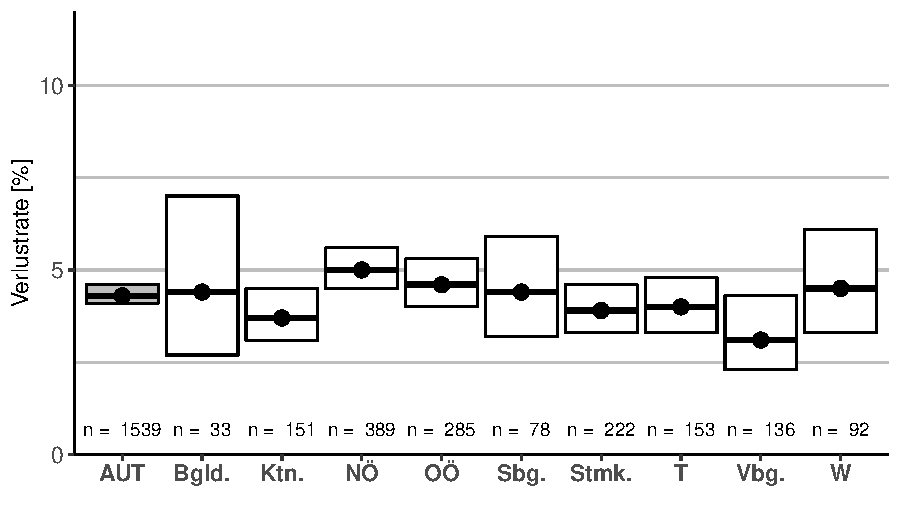
\includegraphics[keepaspectratio,width=0.8\textwidth]{project-U-wintersterblichkeit/figures/plot_queen_states}
  \caption{Höhe der Winterverluste 2019/20 durch unlösbare Königinnen Probleme verursacht für die einzelnen Bundesländer und Österreich gesamt in Prozent ($\pm$95\%KI).}
  \label{fig:u:queen:states}
\end{figure}

\subsubsubsection{Königinnen-Probleme}
\label{ss:koeniginnen_probleme:U}

Die Überlebenschance der Völker hängt in großem Maße auch von der Gesundheit der Königin ab. Die Imkereien wurden deshalb auch über das Auftreten von Königinnen-Problemen befragt und konnten zwischen den vier Antworten „Häufiger``, „Normal``, „Seltener`` und „Weiß nicht`` (im Vergleich zu den Vorjahren) entscheiden. \cref{tab:u:queenproblems} zeigt die Angaben der TeilnehmerInnen von 2013/14 bis 2019/20.
\newline
TeilnehmerInnen die \enquote{Häufiger} diese Probleme beobachteten hatten signifikant höhere Verluste durch \enquote{Unlösbare Königinnenprobleme} mit \confi{6,8}{95}{5,8}{7,9} im Vergleich zu den anderen Gruppen: Normal - \confi{4,3}{95}{4}{4,8}, Seltener - \confi{3,7}{95}{3,2}{4,2}, Weiß nicht - \confi{3,8}{95}{2,8}{5} (\cref{fig:u:queen:problems}-A). Auch bei den Winterverlusten (exkl. \enquote{Unlösbare Königinnenprobleme}) zeigte sich derselbe Trend mit signifikant höheren Verlusten für \enquote{Häufiger} mit \confi{11,2}{95}{8,9}{14} im Vergleich zu den anderen Gruppen: Normal - \confi{7,1}{95}{6,2}{8,1}; Seltener - \confi{7,4}{95}{6,2}{8,7}. Nur die Gruppe \enquote{Weiß nicht} zeigt hier keinen signifikanten Unterschied mit \confi{10,8}{95}{7,9}{14,5} (\cref{fig:u:queen:problems}-B).

\begin{table}[H]
    \centering
    \caption{Art der Teilnahme an der Erhebung der Winterverluste von 2013/14 bis 2019/20 (Anzahl TeilnehmerInnen (\%)).}
    \label{tab:u:queenproblems}
    \begin{tabular}{c|*{3}{rr|}*{2}{r}}
        %\hline
            \multicolumn{1}{c}{} & 
            \multicolumn{2}{c|}{Häufiger} & 
            \multicolumn{2}{c|}{Normal} & 
            \multicolumn{2}{c|}{Seltener} &
            \multicolumn{2}{c}{Weiß nicht}
            \\
        \cline{2-9}
            \multicolumn{1}{c}{Jahr} & 
            \multicolumn{1}{c}{\textit{n}} & 
            \multicolumn{1}{c|}{\%} & 
            \multicolumn{1}{c}{\textit{n}} & 
            \multicolumn{1}{c|}{\%} & 
            \multicolumn{1}{c}{\textit{n}} & 
            \multicolumn{1}{c|}{\%} &
            \multicolumn{1}{c}{\textit{n}} & 
            \multicolumn{1}{c}{\%} \\
        \hline
     2013/14 &  76 &  8,0 & 458 & 48,1 & 212 & 22,2 & 207 & 21,7 \\
     2014/15 & 194 & 16,6 & 513 & 44,0 & 181 & 15,5 & 279 & 23,9 \\
     2015/16 &  63 &  5,2 & 491 & 40,7 & 399 & 33,1 & 253 & 21,0 \\
     2016/17 & 160 & 10,2 & 743 & 47,4 & 396 & 25,2 & 272 & 17,3 \\
     2017/18 &  72 &  6,6 & 529 & 48,4 & 332 & 30,3 & 162 & 14,8 \\
     2018/19 &  95 &  6,2 & 587 & 38,3 & 389 & 25,4 & 463 & 30,2 \\
     2019/20 & 127 & 10,4 & 570 & 46,9 & 354 & 29,1 & 165 & 13,6 \\
     \hline
    \end{tabular}
\end{table}

\begin{figure}[H]
  \centering
  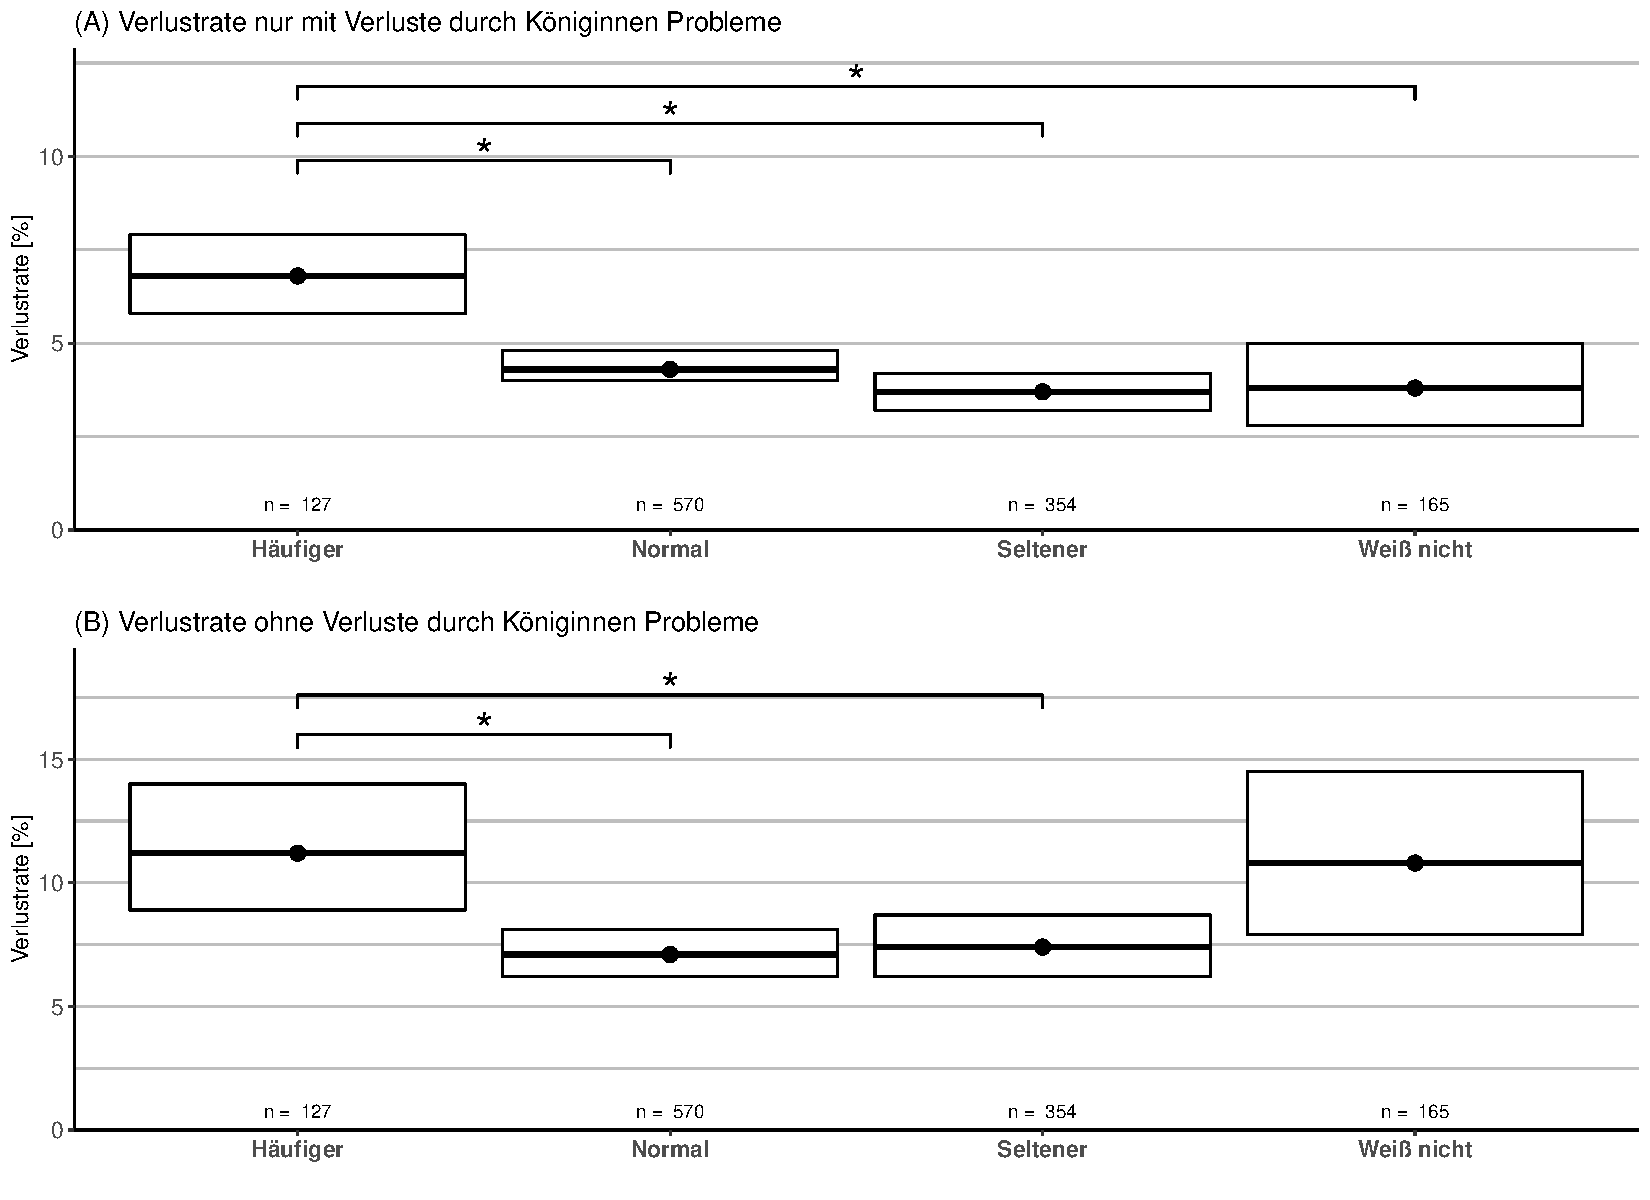
\includegraphics[keepaspectratio,width=0.9\textwidth]{project-U-wintersterblichkeit/figures/plot_queen_subjectiveproblems}
  \caption{Höhe der Winterverluste 2019/20 im Zusammenhang mit den beobachteten Königinnen-Problemen in Prozent ($\pm$95\%KI). (A) nur Verluste durch unlösbare Königinnen Probleme. (B) Winterverluste exklusive den Verlusten durch unlösbare Königinnen-Probleme.}
  \label{fig:u:queen:problems}
\end{figure}


\subsubsubsection{Im Einwinterungsjahr begattete Königin (\enquote{junge Königin})}
\label{ss:junge_koeniginnen:U}

Die ImkerInnen wurden nach der Anzahl ihrer Völker mit junger Königin befragt, um zu sehen, ob sich die Überlebenschancen von Völkern mit einer jungen, das heißt im Jahr 2019 begatteten Königin, im Vergleich zu Völkern mit einer älteren Königin unterscheiden. Hier zeigt sich in unserer Umfrage einen Anteil an jungen Königinnen von 53,1\% in Österreich. Zur Berechnung des Anteils an jungen Königinnen wurden nur TeilnehmerInnen herangezogen welche die Frage \enquote{Wie viele Ihrer eingewinterten Völker hatten eine im Jahr 2019 begattete („junge``) Königin?} beantwortet haben.
\newline
Beim Vergleich der Austauschraten zu Verlusten durch \enquote{Unlösbare Königinnenprobleme} zeigt sich kein signifikanter Unterschied zwischen den Gruppen: 0-25\% (\confi{4}{95}{3,1}{5,1}); 26-50\% (\confi{4,4}{95}{3,9}{4,8}); 51-75\% (\confi{4,6}{95}{4,2}{5,1}) und 76-100\% (\confi{3,8}{95}{3,2}{4,6}) (\cref{fig:u:queen:exchangerate} - A).
\newline
Ein signifikanter positiver Effekt mit weniger Verlusten bei mehr eingesetzten jungen Königinnen zeigt sich aber für die Verlustraten (exkl. \enquote{Unlösbare Königinnenprobleme}). Hier zeigt die Gruppe in der nur \enquote{0-25\%} Königinnen getauscht wurden statistisch signifikant höhere Verlustraten mit \confi{15,3}{95}{12,4}{18,8} im Gegensatz zu den Gruppen in denen prozentual mehr junge Königinnen eingesetzt wurden \enquote{26-50\%} (\confi{8,8}{95}{7,8}{9,9}); \enquote{51-75\%} (\confi{6}{95}{5,1}{7,0}) und \enquote{76-100\%} (\confi{8,0}{95}{6,4}{10,0}). Zusätzlich hat die Gruppe \enquote{26-50\%} statistisch signifikante höhere Verlustraten als die Gruppe \enquote{51-75\%} (\cref{fig:u:queen:exchangerate} - B).

\begin{figure}[H]
  \centering
  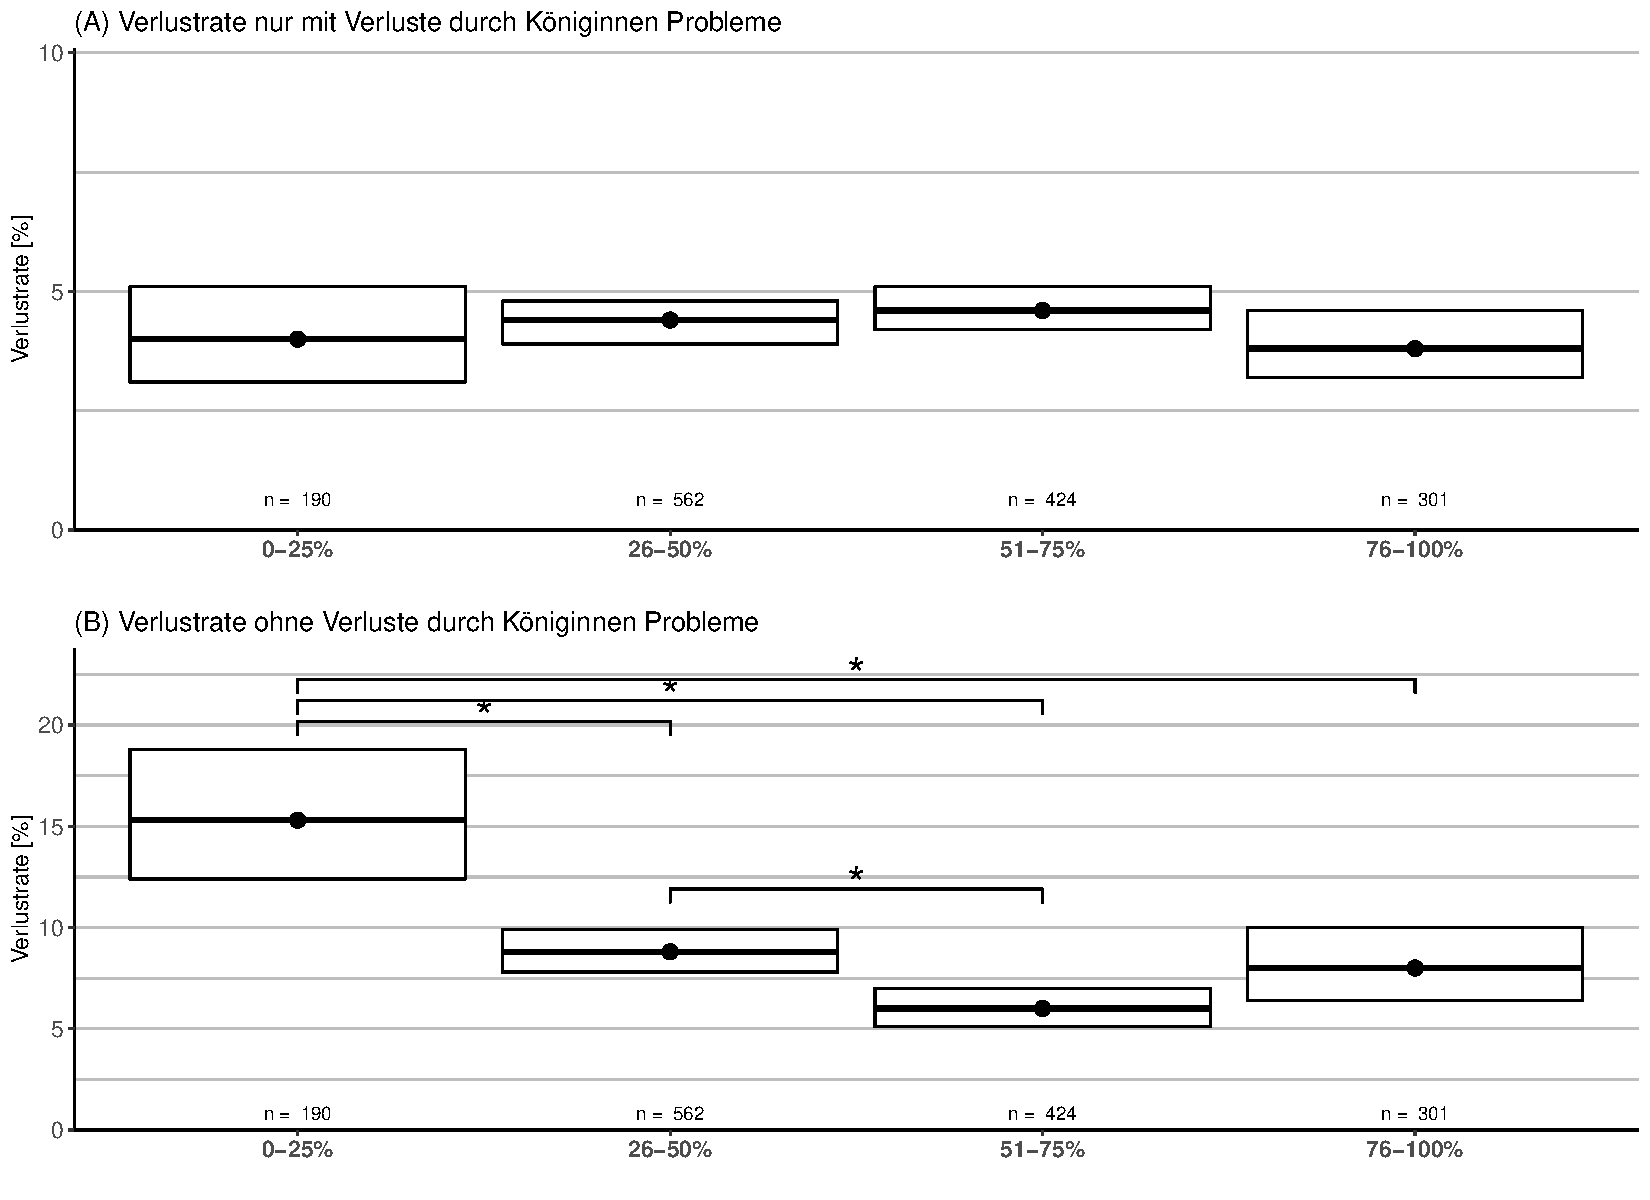
\includegraphics[keepaspectratio,width=0.9\textwidth]{project-U-wintersterblichkeit/figures/plot_queen_exchangerate}
  \caption{Höhe der Winterverluste 2019/20 in Prozent ($\pm$95\%KI) in Abhängigkeit vom Prozentsatz junger Königinnen pro Imkerei. (A) nur Verluste durch unlösbare Königinnen Probleme. (B) Winterverluste exklusive den Verlusten durch unlösbare Königinnen-Probleme.}
  \label{fig:u:queen:exchangerate}
\end{figure}

\subsubsection{Verkrüppelte Flügel}
\label{ss:verkeuppelte_fluegel:U}

In der Erhebung 2019/20 wurde nach dem Auftreten von Bienen mit verkrüppelten Flügeln während der Sammelsaison 2019 gefragt. Nur 2,0\% der Imkereien beobachtete diese \enquote{Häufig}, die Gruppe hatte aber eine statistisch signifikante höhere Verlustrate \confi{19,4}{95}{15,3}{24,3} im Vergleich zur Gruppe \enquote{Wenig} mit \confi{12,6}{95}{11,5}{13,8} sowie wenn keine verkrüppelte Flügeln beobachtet wurden \enquote{Überhaupt nicht} mit \confi{11,5}{95}{10,6}{12,5}. Keinen signifikanten Unterschied gab es zu den Gruppen \enquote{Weiß nicht} (\confi{17,3}{95}{12,3}{23,7}) und \enquote{keine Angaben} (\confi{14}{95}{9,3}{20,4}) \cref{fig:u:queen:crippledbees}).

\begin{figure}[H]
  \centering
  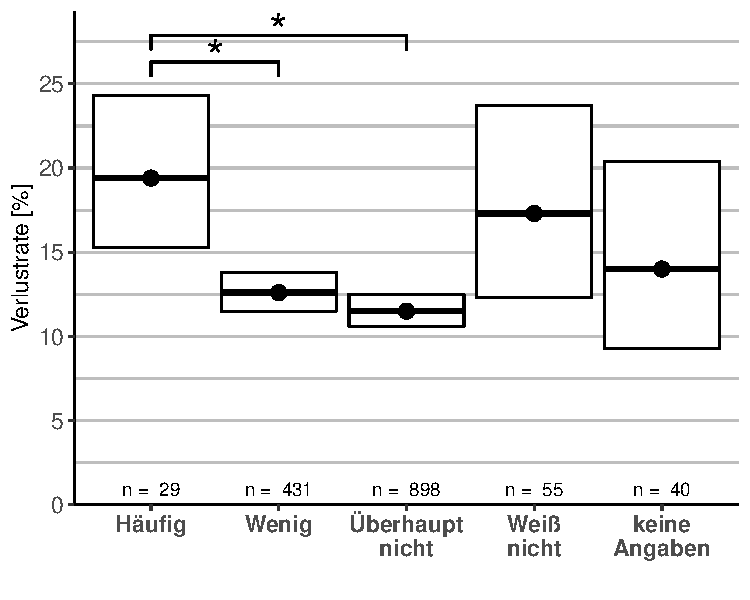
\includegraphics[keepaspectratio,width=0.6\textwidth]{project-U-wintersterblichkeit/figures/plot_factor_crippledbees}
  \caption{Höhe der Winterverluste 2019/20 in Prozent ($\pm$95\%KI) in Abhängigkeit von der Angabe wie Häufig während der Sammelsaison 2019 Bienen mit verkrüppelten Flügeln in den Völkern bemerkt wurden.}
  \label{fig:u:queen:crippledbees}
\end{figure}